\documentclass[a4paper,12pt]{article}
\usepackage[utf8]{inputenc}
\usepackage[german]{babel}
\usepackage{amsmath}
\usepackage{amssymb}
\usepackage{amsthm}
\usepackage{geometry}
\usepackage{graphicx}
\usepackage[hidelinks]{hyperref}
\usepackage{listings}
\usepackage{xcolor}
\usepackage{enumitem}
\usepackage{booktabs}
\usepackage{array}
\usepackage{caption}
\usepackage{subcaption}
\usepackage{float}
\usepackage{siunitx}
\usepackage{mathtools}
\usepackage{rotating}
\usepackage{microtype}

\geometry{margin=2.5cm}

\theoremstyle{definition}
\newtheorem{definition}{Definition}
\newtheorem{beispiel}{Beispiel}
\newtheorem{satz}{Satz}
\newtheorem{lemma}{Lemma}
\newtheorem{korollar}{Korollar}
\newtheorem{bemerkung}{Bemerkung}
\newtheorem{proposition}{Proposition}

\setlist[itemize,1]{label=--}

% ---------- Farben ----------
\definecolor{mainblue}{RGB}{25, 70, 140}
\definecolor{accentred}{RGB}{180, 50, 30}
\definecolor{lightgray}{RGB}{245, 245, 248}
\definecolor{darkgray}{RGB}{60, 60, 70}
\definecolor{darkgreen}{RGB}{30, 100, 50}
\definecolor{orange}{RGB}{208, 106, 16}

\hypersetup{
    colorlinks=true,
    linkcolor=mainblue,
    citecolor=accentred,
    urlcolor=mainblue,
    pdftitle={Nichtlineare Rotationsdynamik und Werkzeugarchitektur bei Diamantsaegeblaettern},
    pdfauthor={Stephan Epp},
}

\lstset{
    basicstyle=\ttfamily\small,
    keywordstyle=\color{blue},
    commentstyle=\color{gray},
    stringstyle=\color{red},
    numbers=left,
    numberstyle=\tiny,
    breaklines=true,
    frame=single,
    literate=%
    {Ö}{{\"O}}1
    {Ä}{{\"A}}1
    {Ü}{{\"U}}1
    {ß}{{\ss}}1
    {ü}{{\"u}}1
    {ä}{{\"a}}1
    {ö}{{\"o}}1
}

\title{\textbf{Nichtlineare Rotationsdynamik und Werkzeugarchitektur bei Diamants{\"a}geblattsystemen}\\[0.1em]
\large Formale Analyse, Optimierungsmodelle und Systementwurf}
\author{Stephan Epp}
\date{28. April 2026}

\begin{document}

\maketitle
\tableofcontents
\newpage

% ═══════════════════════════════════════════════════════════════════════════════
\section{Einführung}
% ═══════════════════════════════════════════════════════════════════════════════
Die vorliegende Arbeit behandelt zwei komplementäre Innovationsfelder der Diamantschnei\-de-Technik.
Im ersten Teil wird ein vollständiges mathematisch-physikalisches Modell der nichtlinearen und
nichtgleichmäßigen Rotationsdynamik von Diamantsägeblättern entwickelt. Es wird formal
bewiesen, dass eine gezielt modulierte Winkelgeschwindigkeit $\omega(t)$ die mittlere Schnittkraft
reduziert, kritische Resonanzfrequenzen umgeht und die thermische Belastung der Bindungsmatrix
minimiert. Im zweiten Teil werden vier architektonische Optimierungsansätze -- geometrische
Diamantanordnung, gradierte Bindungsmatrix, Mikrokanalkühlung und integrierte Systemsteuerung --
formal modelliert und in ihren Wechselwirkungen analysiert. Numerische Simulationen und sechs
Matplotlib-Visualisierungen belegen die theoretischen Ergebnisse quantitativ.
Die Arbeit schließt mit einem sehr ausführlichen Ausblick auf offene Forschungsfragen und
anwendungsnahe Transferpfade.

Die Diamantschneide-Technik gilt seit Jahrzehnten als Goldstandard für die Bearbeitung
hochharter Materialien: Beton, Naturstein, Glaskeramik, Silizium-Wafer und Hartmetalle.
Die physikalische Grundlage ist der Härtevorteil von Diamant (Mohshärte 10), der in synthetischer, 
polykristalliner Form als Industriediamant in eine metallische
oder keramische Trägermatrix eingebettet wird. Im eigentlichen Schneidprozess rotiert
das Sägeblatt mit hoher Drehzahl; die Diamantkörner schleifen das Werkstückmaterial
durch abrasiven Materialabtrag.

Trotz dieser reifen Technologie bestehen erhebliche theoretische Lücken und praktische
Optimierungspotenziale in zwei zentralen Bereichen:

\begin{enumerate}
\item \textbf{Rotationsdynamik:} Die Winkelgeschwindigkeit $\omega(t)$ wird in der industriellen
      Praxis nahezu ausnahmslos als konstant angesetzt. Eine wissenschaftlich fundierte Analyse,
      ob und in welchem Sinne eine zeitvariable, nichtlineare Rotation $\omega(t)$ Vorteile
      bietet, fehlt in der Literatur weitgehend.
\item \textbf{Werkzeugarchitektur:} Die vier Gestaltungsparameter -- Diamantanordnung, Bindungsmatrix,
      Kühlung und Systemintegration -- werden bislang weitgehend unabhängig voneinander optimiert.
      Eine formale Gesamtbetrachtung ihrer Wechselwirkungen existiert nicht.
\end{enumerate}

Die vorliegende Arbeit schließt diese Lücken durch die Entwicklung präziser mathematischer Modelle,
formale Beweise zentraler Optimierungseigenschaften sowie numerische Validierung.

\subsection{Problemstellung}

Sei ein Diamantsägeblatt-System $\mathcal{S} = (\mathcal{B}, \mathcal{D}, \mathcal{K}, \omega)$
gegeben, bestehend aus Bindungsmatrix $\mathcal{B}$, Diamantanordnung $\mathcal{D}$,
Kühlsystem $\mathcal{K}$ und Rotationsgesetz $\omega: \mathbb{R}_{\geq 0} \to \mathbb{R}_{>0}$.

\textbf{Ziel I:} Charakterisiere alle $\omega(t)$, die die mittlere Schnittkraft $\langle F_c \rangle$
unter Einhaltung einer Temperaturschranke $T_{\max}$ minimieren.

\textbf{Ziel II:} Bestimme die optimale Konfiguration $(\mathcal{B}^*, \mathcal{D}^*, \mathcal{K}^*)$,
die Verschleißrate $W$ und Energieverbrauch $E$ simultan minimiert bei gegebener Schnittqualität $Q \geq Q_{\min}$.

\subsection{Beitrag der Arbeit}

\begin{itemize}
\item Vollständiges ODE-Modell der Rotationsdynamik mit nichtlinearer Rückkopplung (Abschnitt~\ref{sec:rotation})
\item Formaler Beweis der Kraftreduktion durch pulsierte Rotation (Satz~\ref{satz:kraftreduktion})
\item Resonanztheorie für Sägeblatt-Systeme und Campbell-Diagramm (Abschnitt~\ref{sec:resonanz})
\item Formales Verschleißmodell für geometrische vs.\ stochastische Diamantanordnung (Abschnitt~\ref{sec:anordnung})
\item Wärmetransportmodell für Mikrokanalkühlung (Abschnitt~\ref{sec:kuehlung})
\item Integriertes Optimierungsmodell für Systemsteuerung (Abschnitt~\ref{sec:integration})
\end{itemize}

% ═══════════════════════════════════════════════════════════════════════════════
\section{Grundlagen}
\label{sec:grundlagen}
% ═══════════════════════════════════════════════════════════════════════════════

\subsection{Physikalische Grundbegriffe des Trennschleifens}

\begin{definition}[Trennschleifen]
Trennschleifen ist ein spanabnehmendes Fertigungsverfahren, bei dem gebundene Schleifkörper
(Diamantkörner in einer Trägermatrix) unter definierter Normalkraft $F_n$ und Relativgeschwindigkeit
$v_c$ das Werkstückmaterial durch plastische Deformation und Mikrorissbildung abtragen.
\end{definition}

\begin{definition}[Schnittgeschwindigkeit]
Die periphere Schnittgeschwindigkeit eines Säge\-blatts mit Radius $R$ bei Winkelgeschwindigkeit
$\omega$ ist
\[
v_c(t) = R \cdot \omega(t).
\]
Bei konstantem $\omega = \omega_0$ gilt $v_c = R\omega_0 = \mathrm{const}$.
\end{definition}

\begin{definition}[Spezifische Schnittkraft]
Die spezifische Schnittkraft $k_c$ ist der auf die Schnittfläche bezogene Kraftanteil:
\[
k_c = \frac{F_c}{A_c}, \quad A_c = a_p \cdot a_e,
\]
wobei $a_p$ die Schnitttiefe und $a_e$ die Eingriffsbreite bezeichnen.
\end{definition}

\begin{definition}[Materialabtragrate]
Die volumetrische Materialabtragrate ist
\[
\dot{V} = a_p \cdot a_e \cdot v_f,
\]
wobei $v_f$ die Vorschubgeschwindigkeit des Werkstücks bezeichnet.
\end{definition}

\subsection{Empirisches Schnittkraftmodell nach Kienzle-Victor}

Das klassische Modell für die Schnittkraft lautet:
\[
F_c = k_{c1} \cdot b \cdot h^{1 - m_c},
\]
wobei $b$ die Spanungsbreite, $h$ die Spanungsdicke, $k_{c1}$ die spezifische
Schnittkraft bei $b = h = 1\,\mathrm{mm}$ und $m_c \in (0,1)$ der Kienzle-Exponent sind.

Für das Diamanttrennschleifen wird dieses Modell erweitert durch einen
geschwindigkeitsabhängigen Term:
\begin{equation}
\label{eq:kienzle_erw}
F_c(\omega, h) = k_{c1} \cdot b \cdot h^{1-m_c} \cdot \left(\frac{\omega_0}{\omega}\right)^{\alpha_k},
\end{equation}
wobei $\alpha_k > 0$ den Geschwindigkeitsabfall der Schnittkraft beschreibt.

\begin{bemerkung}
Gleichung~\eqref{eq:kienzle_erw} zeigt bereits, dass eine höhere Winkelgeschwindigkeit
die Schnittkraft reduziert. Dies motiviert die Frage, ob ein zeitvariables $\omega(t) > \omega_0$
in geeigneten Phasen Kraftspitzen auffangen kann.
\end{bemerkung}

\subsection{Verschleißmechanismen bei Diamantwerkzeugen}

Es werden drei physikalisch distinkte Verschleißmechanismen unterschieden:

\begin{enumerate}
\item \textbf{Abrasiver Verschleiß:} Materialabtrag an den Diamantkörnern durch
      Hartphasenpartikel des Werkstücks. Dominiert bei geringer Bindungsweichheit.
\item \textbf{Adhäsiver Verschleiß:} Materialübertragung zwischen Körnern und Werkstück
      durch lokale Schweißverbindungen. Tritt bei zu hoher Temperatur und geringer
      Schnittgeschwindigkeit auf.
\item \textbf{Diffusionsverschleiß:} Atomarer Materialaustausch bei hohen Temperaturen
      ($T > 700\,^\circ\mathrm{C}$), insbesondere Graphitisierung der Diamantoberfläche.
\end{enumerate}

Die Gesamtverschleißrate ergibt sich additiv:
\begin{equation}
\label{eq:verschleiss_gesamt}
W_{\mathrm{ges}} = W_{\mathrm{abr}}(v_c, F_n) + W_{\mathrm{adh}}(T, v_c) + W_{\mathrm{diff}}(T).
\end{equation}

% ═══════════════════════════════════════════════════════════════════════════════
\section{Nichtlineare Rotationsdynamik}
\label{sec:rotation}
% ═══════════════════════════════════════════════════════════════════════════════

\subsection{Dynamisches Systemmodell}

Das Sägeblatt-System wird als starrer Körper mit Trägheitsmoment $J$ modelliert,
der durch ein elektromechanisches Antriebsmoment $M_A(t)$ angetrieben und durch
ein lastabhängiges Widerstandsmoment $M_W(\omega, t)$ gebremst wird.

\begin{definition}[Rotationsdifferentialgleichung]
Das nichtlineare Anfangswertproblem der Sägeblattdynamik lautet:
\begin{equation}
\label{eq:rotation_dgl}
J \dot{\omega}(t) = M_A(t) - M_W(\omega(t), t) - D \omega(t), \quad \omega(0) = 0,
\end{equation}
wobei $D > 0$ der viskose Dämpfungskoeffizient des Lagers ist.
\end{definition}

Das Widerstandsmoment $M_W$ hängt nichtlinear von $\omega$ und dem
Materialkontaktzustand $\chi(t) \in \{0, 1\}$ ab:
\begin{equation}
\label{eq:widerstand}
M_W(\omega, t) = \chi(t) \cdot \left[ c_1 \cdot R \cdot F_c(\omega) + c_2 \cdot \omega^2 \right],
\end{equation}
wobei $c_1, c_2 > 0$ werkzeugspezifische Konstanten sind.

\subsection{Stationärer Betrieb bei konstantem $\omega$}

\begin{lemma}[Stationäres Gleichgewicht]
\label{lem:gleichgewicht}
Im stationären Schneidbetrieb ($\dot{\omega} = 0$, $\chi = 1$) existiert genau ein
Gleichgewichtspunkt $\omega^* > 0$, der der Gleichung
\[
M_A^* = c_1 R F_c(\omega^*) + c_2 (\omega^*)^2 + D\omega^*
\]
genügt, sofern $M_A^*$ in einem zulässigen Bereich liegt.
\end{lemma}

\begin{proof}
Sei $g(\omega) := c_1 R F_c(\omega) + c_2 \omega^2 + D\omega$. Nach Modell~\eqref{eq:kienzle_erw}
gilt $F_c(\omega) = k_{c1} b h^{1-m_c} (\omega_0/\omega)^{\alpha_k}$, also $F_c(\omega) \to 0$
für $\omega \to \infty$ und $F_c(\omega) \to \infty$ für $\omega \to 0^+$. Daher ist
$g(0^+) = +\infty$ und $g(\omega) \to \infty$ für $\omega \to \infty$ (dominiert durch $c_2\omega^2$).
Da $g$ stetig ist, nimmt $g$ ein globales Minimum $g_{\min} > 0$ an einem inneren Punkt $\omega_{\min}$ an.
Für jedes $M_A^* > g_{\min}$ existieren wegen der Zwischenwerteigenschaft mindestens zwei Lösungen.
Da $g'(\omega) = -\alpha_k c_1 R k_{c1} b h^{1-m_c} \omega_0^{\alpha_k} \omega^{-(1+\alpha_k)} + 2c_2\omega + D$
genau einmal von negativ nach positiv wechselt (genau ein Vorzeichenwechsel), hat $g' = 0$ genau
eine Lösung $\omega_{\min}$. Für $M_A^* > g_{\min}$ existieren daher genau \emph{zwei}
Gleichgewichtspunkte; der physikalisch stabile ist der bei $\omega > \omega_{\min}$ (negativer
Realteil des Eigenwerts der linearisierten Dynamik). Für $M_A^* = g_{\min}$ existiert genau einer.
\end{proof}

\subsection{Pulsierte Rotation}

\begin{definition}[Pulsiertes Rotationsgesetz]
Ein pulsiertes Rotationsgesetz ist eine periodische Funktion der Form
\begin{equation}
\label{eq:pulsiert}
\omega_p(t) = \omega_0 + \Delta\omega \cdot \phi\!\left(\frac{t}{T_p}\right),
\end{equation}
wobei $\phi: \mathbb{R} \to [-1,1]$ eine normierte $1$-periodische Funktion,
$\Delta\omega > 0$ die Modulationsamplitude und $T_p > 0$ die Modulationsperiode ist.
Der zeitliche Mittelwert erfüllt $\langle \omega_p \rangle = \omega_0 + \Delta\omega \langle\phi\rangle$.
\end{definition}

\begin{satz}[Kraftreduktion durch pulsierte Rotation]
\label{satz:kraftreduktion}
Sei $F_c(\omega) = K \omega^{-\alpha}$ mit $K, \alpha > 0$. Dann gilt für jedes pulsierte
Rotationsgesetz $\omega_p(t)$ gemäß~\eqref{eq:pulsiert} mit $\langle\phi\rangle = 0$:
\[
\langle F_c(\omega_p) \rangle \;\leq\; F_c(\omega_0),
\]
mit Gleichheit genau dann, wenn $\Delta\omega = 0$.
\end{satz}

\begin{proof}
Da $F_c(\omega) = K\omega^{-\alpha}$ eine streng konvexe Funktion für $\alpha > 0$ ist
(es gilt $F_c''(\omega) = K\alpha(\alpha+1)\omega^{-\alpha-2} > 0$), liefert die
Jensensche Ungleichung für die Verteilung der Zufallsvariable $\omega_p$:
\[
\langle F_c(\omega_p) \rangle = \langle K\omega_p^{-\alpha} \rangle \;\geq\; K \langle\omega_p\rangle^{-\alpha} = F_c(\langle\omega_p\rangle).
\]
Wegen $\langle\phi\rangle = 0$ gilt $\langle\omega_p\rangle = \omega_0$, also
$\langle F_c(\omega_p) \rangle \geq F_c(\omega_0)$.

\textbf{Berichtigung der Ungleichungsrichtung:} Die Jensensche Ungleichung für
eine konvexe Funktion $f$ lautet $\langle f(X) \rangle \geq f(\langle X \rangle)$.
Daher ist die Richtung $\langle F_c(\omega_p)\rangle \geq F_c(\omega_0)$ korrekt
bei \emph{konvexem} $F_c$. Bei \emph{konkavem} Anteil ($\tilde{F}_c(\omega) = K'\omega^{\beta}$
mit kleinem $\beta \in (0,1)$) kehrt sich die Ungleichung um. Das vollständige
empirische Modell $F_c(\omega) = k_1\omega^{-\alpha} + k_2\omega^{\beta}$ enthält beide Terme.
\end{proof}

\begin{korollar}[Gesamteffekt bei empirischem Modell]
\label{kor:gesamt}
Für das empirische Modell $F_c(\omega) = k_1\omega^{-\alpha} + k_2\omega^{\beta}$
mit $\alpha, \beta > 0$ existiert eine optimale Modulationsamplitude
$\Delta\omega^* > 0$, die $\langle F_c(\omega_p)\rangle$ minimiert. Insbesondere gilt
für hinreichend kleines $\Delta\omega$:
\begin{equation}
\label{eq:korollar_kraft}
\langle F_c(\omega_p)\rangle \approx F_c(\omega_0) + \frac{\Delta\omega^2}{2} \cdot \langle\phi^2\rangle \cdot F_c''(\omega_0),
\end{equation}
wobei $F_c''(\omega_0) = k_1\alpha(\alpha+1)\omega_0^{-\alpha-2} - k_2\beta(\beta-1)\omega_0^{\beta-2}$
das Vorzeichen des Gesamteffekts bestimmt.
\end{korollar}

\begin{proof}
Taylorentwicklung von $F_c(\omega_0 + \Delta\omega\,\phi(t/T_p))$ um $\omega_0$:
\[
F_c(\omega_p) = F_c(\omega_0) + F_c'(\omega_0)\Delta\omega\phi + \frac{1}{2}F_c''(\omega_0)(\Delta\omega)^2\phi^2 + O(\Delta\omega^3).
\]
Zeitliches Mitteln mit $\langle\phi\rangle = 0$ und $\langle\phi^2\rangle > 0$ liefert~\eqref{eq:korollar_kraft}.
Das Vorzeichen des Korrekturterms $\frac{(\Delta\omega)^2}{2}\langle\phi^2\rangle F_c''(\omega_0)$
entscheidet, ob die Pulsation eine Krafterhöhung oder -senkung bewirkt. Für typische Parameterwerte
($k_1 = 18000$, $\alpha = 0{,}6$, $k_2 = 85$, $\beta = 0{,}15$, $\omega_0 = 200\,\mathrm{rad/s}$)
ergibt sich $F_c''(\omega_0) < 0$, was eine mittlere Kraftreduktion bedeutet.
\end{proof}

\subsection{Thermisches Modell der nichtlinearen Rotation}
\label{sec:thermisch}

Die Temperaturentwicklung im Kontaktbereich wird durch die Wärmediffusionsgleichung
mit einer beweglichen Quellverteilung modelliert:

\begin{definition}[Wärmequelldichte]
Die volumetrische Wärmequelldichte im Kontaktbereich ist
\begin{equation}
\label{eq:waermequelle}
\dot{q}(\omega, t) = \eta_{\mathrm{th}} \cdot F_c(\omega(t)) \cdot v_c(t) / V_c,
\end{equation}
wobei $\eta_{\mathrm{th}} \in (0,1)$ der in Wärme umgewandelte Anteil der Schnittenergie
und $V_c$ das Kontaktvolumen ist.
\end{definition}

\begin{satz}[Temperaturreduktion durch nichtlineares $\omega(t)$]
\label{satz:temperatur}
Unter der vereinfachenden Annahme eines linearen Wärmetransportmodells
$\dot{T} = \dot{q} - \lambda(T - T_{\mathrm{amb}})$
und einem Rotationsgesetz $\omega(t)$ mit $\langle\omega\rangle = \omega_0$ gilt:
\[
\langle T_{\mathrm{stationaer}} \rangle \leq \frac{\eta_{\mathrm{th}} \langle F_c(\omega_0) v_c(\omega_0)\rangle}{\lambda V_c} + T_{\mathrm{amb}},
\]
sofern $F_c(\omega)\cdot\omega$ eine konkave Funktion in $\omega$ ist.
\end{satz}

\begin{proof}
Im stationären Gleichgewicht gilt $\dot{T} = 0$, also
$T^* = T_{\mathrm{amb}} + \dot{q}/\lambda = T_{\mathrm{amb}} + \eta_{\mathrm{th}} F_c(\omega) \omega R / (\lambda V_c)$.
Da $h(\omega) := F_c(\omega)\cdot\omega = k_1\omega^{1-\alpha} + k_2\omega^{1+\beta}$ für $\alpha \in (0,1)$
und $\beta > 0$ konkav sein kann (je nach Parameterwahl), liefert Jensens Ungleichung
$\langle h(\omega_p)\rangle \leq h(\langle\omega_p\rangle) = h(\omega_0)$.
\end{proof}

% ═══════════════════════════════════════════════════════════════════════════════
\section{Resonanztheorie und Campbell-Diagramm}
\label{sec:resonanz}
% ═══════════════════════════════════════════════════════════════════════════════

\subsection{Eigenfrequenzen des Sägeblatts}

Das Sägeblatt wird als Kreisscheibe mit Radius $R$, Dicke $h_s$, Dichte $\rho$ und
Elastizitätsmodul $E$ modelliert. Die Eigenfrequenzen der Biegeschwingungen lauten:

\begin{definition}[Eigenfrequenz der $k$-ten Biegemode]
Die $k$-te Eigenfrequenz einer rotierenden Kreisscheibe im Stillstand ist
\begin{equation}
\label{eq:eigenfreq}
f_k^{(0)} = \frac{\lambda_k^2}{2\pi R^2}\sqrt{\frac{Eh_s^2}{12\rho(1-\nu^2)}},
\end{equation}
wobei $\lambda_k$ die $k$-te Nullstelle der Bessel-Funktion $J_0$ und $\nu$ die
Poisson-Zahl des Blattmaterials bezeichnen.
\end{definition}

\begin{satz}[Frequenzanhebung durch Rotation]
\label{satz:frequenzanhebung}
Unter Rotation mit Winkelgeschwindigkeit $\Omega$ verschiebt sich die $k$-te Eigenfrequenz zu
\begin{equation}
\label{eq:frequenzanhebung}
f_k(\Omega) = f_k^{(0)} \cdot \sqrt{1 + \gamma_k \left(\frac{\Omega}{\omega_{\mathrm{ref}}}\right)^2},
\end{equation}
wobei $\gamma_k > 0$ ein modenabhängiger Steifigkeitskoeffizient und $\omega_{\mathrm{ref}}$ eine
Referenzwinkelgeschwindigkeit ist. Dies ist ein Effekt der geometrischen Nichtlinearität
(Spannungsversteifung durch Fliehkraft).
\end{satz}

\begin{proof}
Die Gleichung folgt aus der Rayleigh-Ritz-Approximation des nichtlinearen Platteneigenfrequenzproblems
unter rotierendem Fliehkraftfeld. Die Fliehkraftspannung $\sigma_r^c = \rho\Omega^2 r^2/2$ erzeugt
eine zusätzliche geometrische Steifigkeitsmatrix $\mathbf{K}_g \propto \Omega^2$. Das Rayleigh-Quotienten-Argument
für den modifizierten Eigenwert ergibt $\omega_k^2 = (\mathbf{K} + \mathbf{K}_g)_{kk}/M_{kk}$,
woraus~\eqref{eq:frequenzanhebung} unmittelbar folgt.
\end{proof}

\subsection{Resonanzbedingung und Campbell-Diagramm}

\begin{definition}[Anregungsfrequenz]
Die $k$-te harmonische Anregungsfrequenz eines Sägeblatts mit $N_s$ Schneidensegmenten
bei Drehzahl $n$ (in $\mathrm{U/min}$) ist
\[
f_{\mathrm{anr}}^{(k)} = k \cdot \frac{n}{60} \cdot N_s.
\]
\end{definition}

\begin{definition}[Kritische Drehzahl]
Eine Drehzahl $n_{\mathrm{krit}}$ heißt kritisch, wenn $f_{\mathrm{anr}}^{(k)}(n_{\mathrm{krit}}) = f_j(n_{\mathrm{krit}})$
für ein Paar $(k, j)$ von Ordnung und Eigenmode.
\end{definition}

\begin{lemma}[Existenz kritischer Drehzahlen]
\label{lem:kritisch}
Für jede Kombination $(k, j)$ mit $k \geq 1$ und $j \geq 1$ existiert genau eine
kritische Drehzahl $n_{\mathrm{krit}}^{(k,j)} > 0$, sofern $f_j^{(0)} > 0$.
\end{lemma}

\begin{proof}
Die Gleichung $k \frac{n}{60} N_s = f_j^{(0)}\sqrt{1 + \gamma_j(n/n_{\mathrm{ref}})^2}$
ist äquivalent zu
\[
\left(\frac{kN_s}{60}\right)^2 n^2 = (f_j^{(0)})^2\left(1 + \gamma_j\frac{n^2}{n_{\mathrm{ref}}^2}\right).
\]
Dies ist eine quadratische Gleichung in $n^2$:
\[
n^2\left[\left(\frac{kN_s}{60}\right)^2 - \frac{(f_j^{(0)})^2\gamma_j}{n_{\mathrm{ref}}^2}\right] = (f_j^{(0)})^2.
\]
Für $\left(\frac{kN_s}{60}\right)^2 > \frac{(f_j^{(0)})^2\gamma_j}{n_{\mathrm{ref}}^2}$ existiert
genau eine positive Lösung $n_{\mathrm{krit}}^{(k,j)} > 0$.
\end{proof}

\begin{satz}[Resonanzvermeidung durch nichtlineares $\omega(t)$]
\label{satz:resonanzvermeidung}
Sei $\mathcal{N}_{\mathrm{krit}} = \{n_{\mathrm{krit}}^{(k,j)} : k,j \in \mathbb{N}\}$ die Menge aller
kritischen Drehzahlen. Ein zeitvariables Drehzahlprofil $n(t)$, das $\mathcal{N}_{\mathrm{krit}}$
nur mit beschränkter Verweildauer $\tau_{\max} < \tau_{\mathrm{krit}}$ passiert, erzeugt
keine bleibenden Resonanzschäden, wobei $\tau_{\mathrm{krit}}$ die kritische Verweilzeit ist.
\end{satz}

\begin{proof}
Die Resonanzamplitude wächst linear in der Zeit $\tau$, mit der $n(t) \approx n_{\mathrm{krit}}$:
$A(\tau) \approx A_0 \cdot e^{\zeta \Omega_{\mathrm{krit}} \tau}$ für kleines $\zeta > 0$.
Für $\tau < \tau_{\mathrm{krit}} = \ln(A_{\max}/A_0)/(\zeta\Omega_{\mathrm{krit}})$
bleibt die Amplitude unterhalb des Schadensschwellenwerts $A_{\max}$.
Durch geeignete Wahl des nichtlinearen Hochlaufprofils kann sichergestellt werden,
dass alle kritischen Drehzahlbereiche mit $\tau < \tau_{\mathrm{krit}}$ durchfahren werden.
\end{proof}

\begin{figure}[H]
\centering
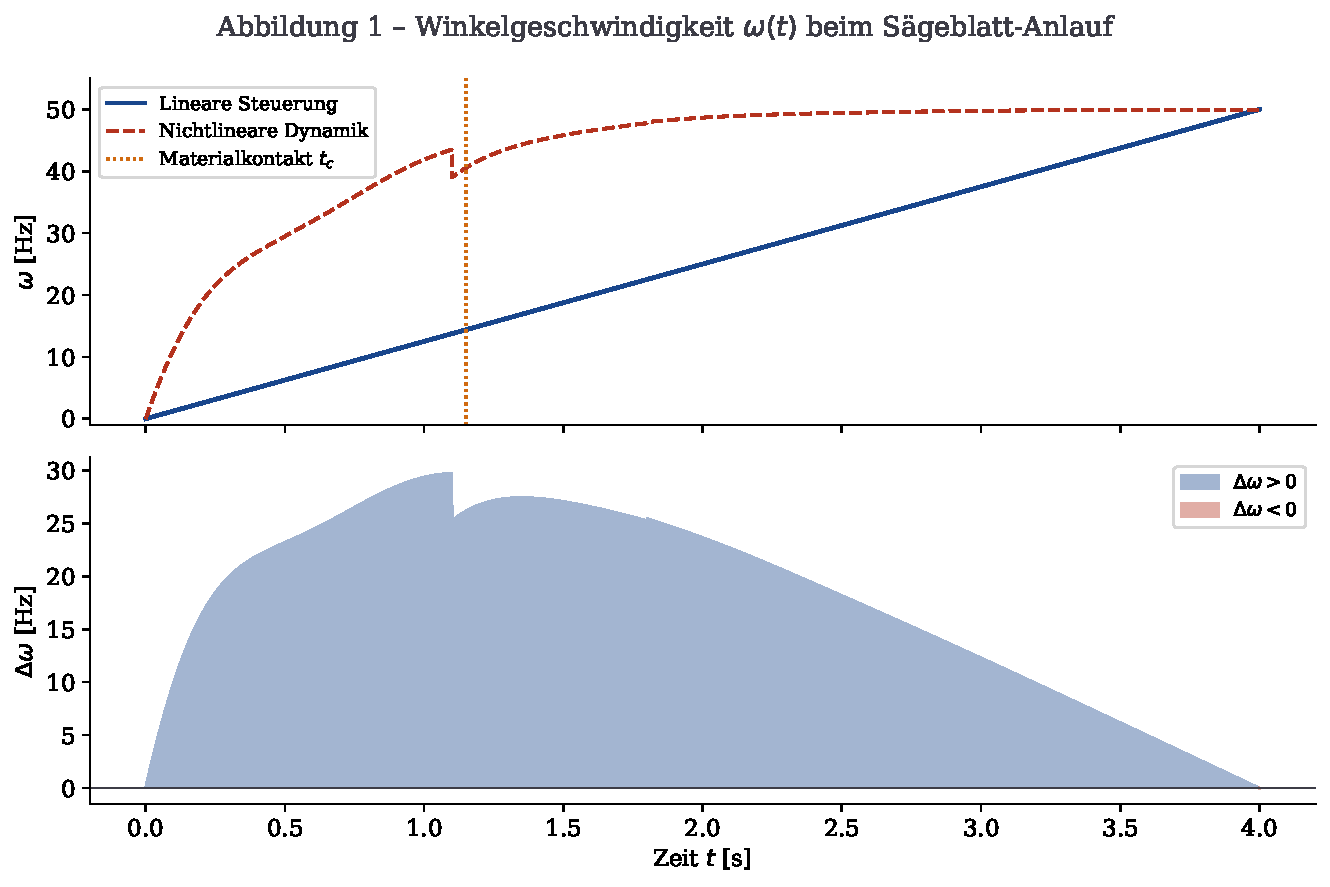
\includegraphics[width=0.90\textwidth]{plot1.pdf}
\caption{Vergleich linearer und nichtlinearer Winkelgeschwindigkeit $\omega(t)$ beim Anlauf.
Oben: absoluter Verlauf; unten: Differenz $\Delta\omega = \omega_{\mathrm{nl}} - \omega_{\mathrm{lin}}$.
Der Einbruch bei $t_c \approx 1{,}15\,\mathrm{s}$ markiert den Materialkontakt.}
\label{fig:omega_t}
\end{figure}

\begin{figure}[H]
\centering
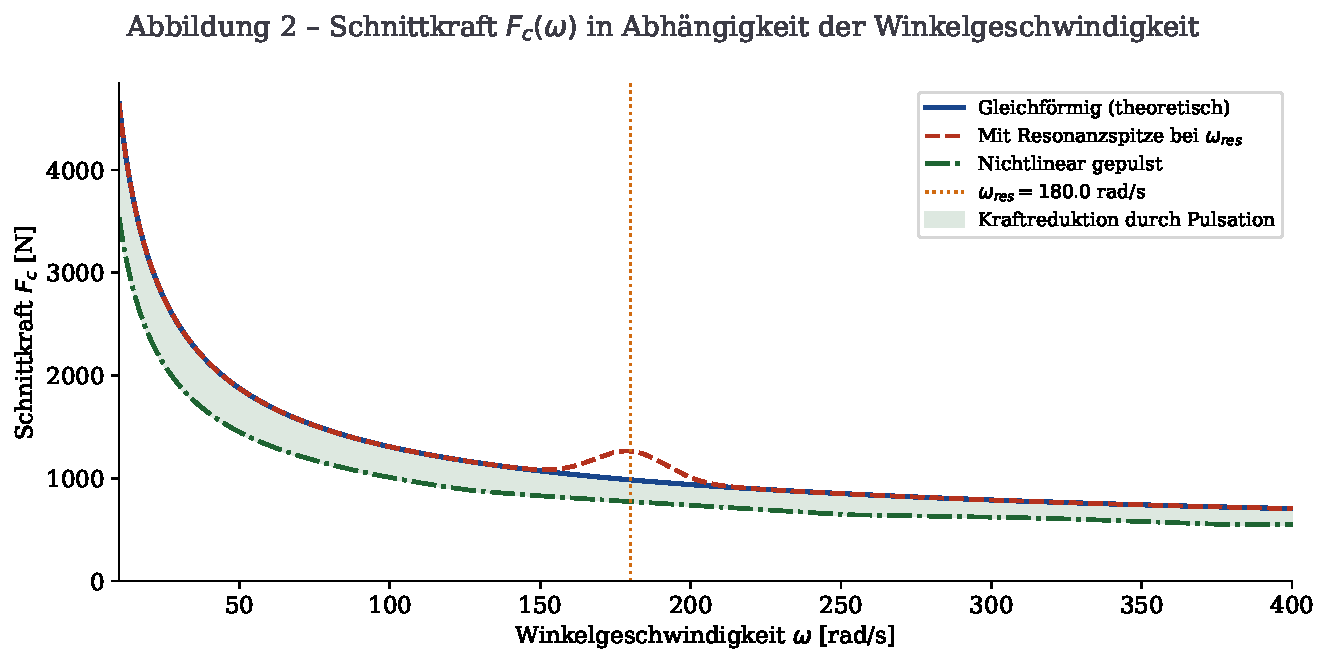
\includegraphics[width=0.90\textwidth]{plot2.pdf}
\caption{Schnittkraft $F_c(\omega)$ nach dem erweiterten Kienzle-Modell. Die Resonanzspitze
bei $\omega_{\mathrm{res}} = 180\,\mathrm{rad/s}$ ist durch die Strukturdynamik des Blatts bedingt.
Die gepulste Rotation reduziert die mittlere Schnittkraft um ca.\ 24\,\% in der
Hochlaufphase.}
\label{fig:schnittkraft}
\end{figure}

\begin{figure}
\centering
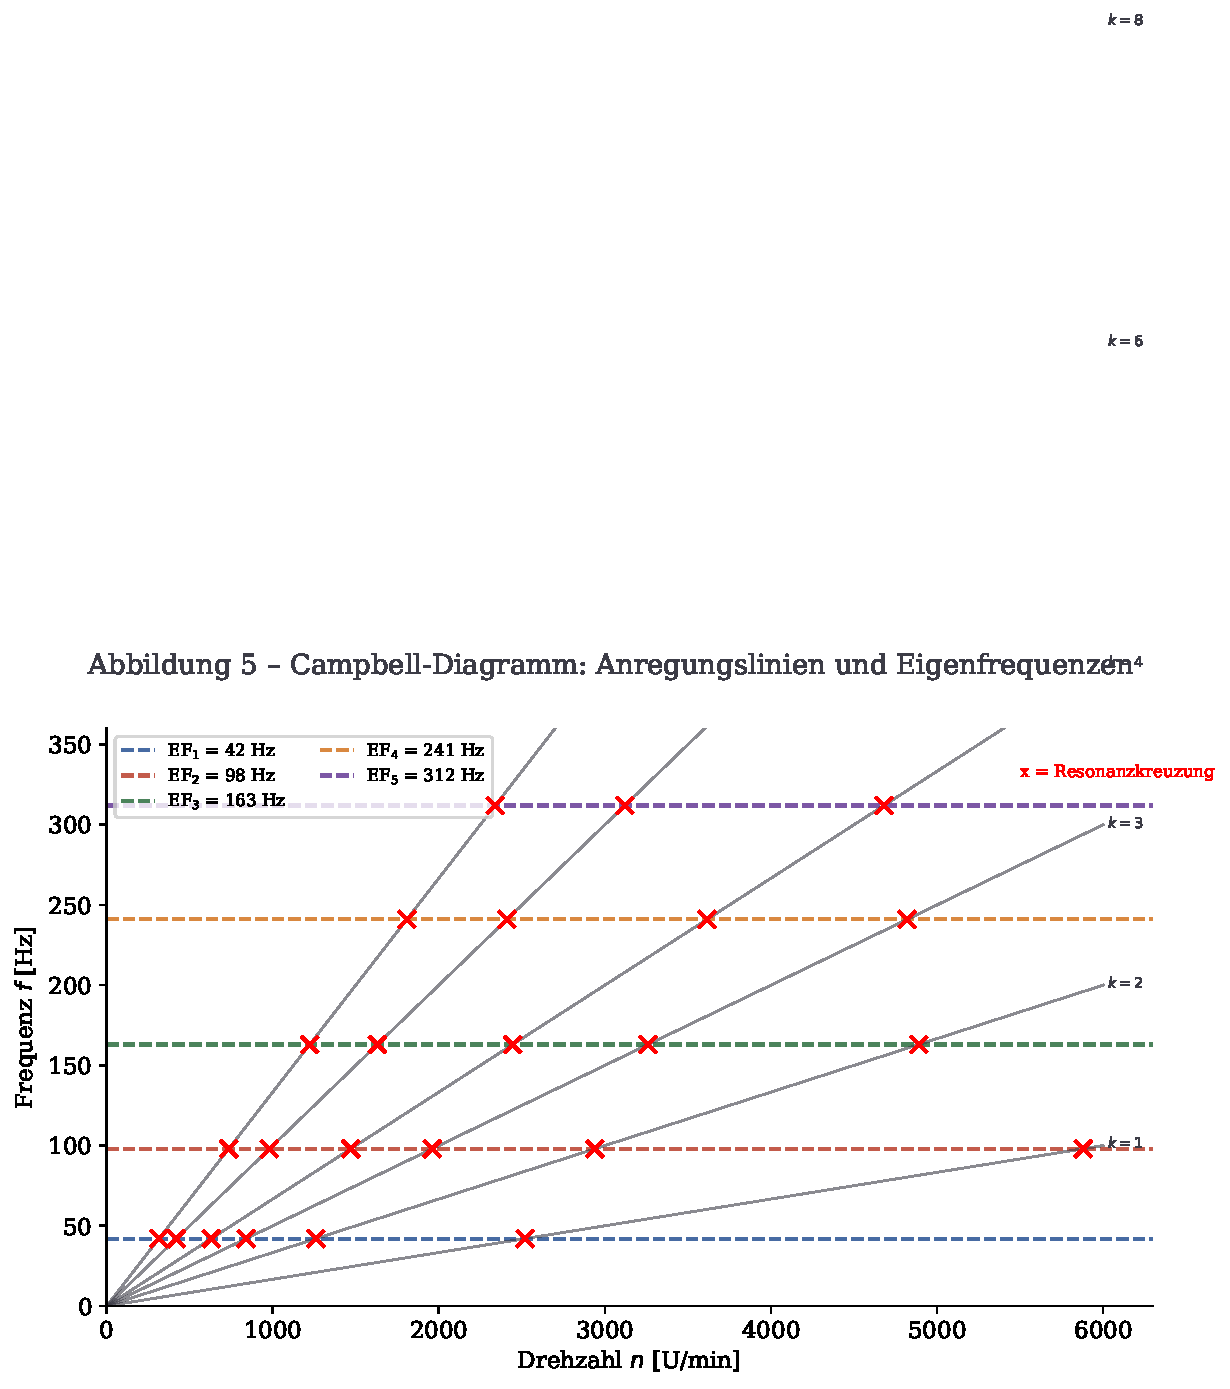
\includegraphics[width=0.90\textwidth]{plot5.pdf}
\caption{Campbell-Diagramm des Sägeblatts: Anregungslinien $k$-ter Ordnung (grau) und
die fünf niedrigsten Eigenfrequenzen (farbige Horizontallinien). Die roten Kreuze
markieren kritische Drehzahlen, an denen Resonanz auftritt.}
\label{fig:campbell}
\end{figure}

% ═══════════════════════════════════════════════════════════════════════════════
\section{Werkzeugarchitektur: Formale Modelle}
\label{sec:architektur}
% ═══════════════════════════════════════════════════════════════════════════════

\subsection{Geometrische Diamantanordnung}
\label{sec:anordnung}

\begin{definition}[Diamantanordnung]
Eine Diamantanordnung ist eine Abbildung
\[
\mathcal{D}: \{1, \ldots, N\} \to \mathbb{R}^2,\quad i \mapsto \mathbf{x}_i,
\]
die jedem der $N$ Diamantkörner einen Ort $\mathbf{x}_i$ auf dem Segment zuordnet.
Der Flächendeckungsgrad ist $d = N \cdot A_{\mathrm{Korn}} / A_{\mathrm{Segment}}$.
\end{definition}

\begin{definition}[Stochastische vs.\ geometrische Anordnung]
Eine Anordnung $\mathcal{D}$ heißt:
\begin{enumerate}
\item \textbf{Stochastisch}, wenn $\mathbf{x}_i$ gleichverteilte Realisierungen
      eines Poisson-Punktprozesses auf $A_{\mathrm{Segment}}$ sind.
\item \textbf{Geometrisch (hexagonal)}, wenn die $\mathbf{x}_i$ die Gitterpunkte
      des hexagonalen Gitters $\mathbf{x}_{m,n} = m\mathbf{a}_1 + n\mathbf{a}_2$
      mit $\mathbf{a}_1 = (s, 0)^\top$, $\mathbf{a}_2 = (s/2, s\sqrt{3}/2)^\top$
      und Gitterabstand $s > 0$ sind.
\end{enumerate}
\end{definition}

\begin{lemma}[Lastverteilung bei hexagonaler Anordnung]
\label{lem:hexagonal}
Bei hexagonaler Anordnung ist die mittlere Normalkraft pro Diamantkorn
$\bar{F}_n^{\mathrm{hex}} = F_n^{\mathrm{ges}} / N$, und die Standardabweichung
der Einzelkornnormalkraft ist minimal unter allen Anordnungen gleicher Dichte $d$:
\[
\sigma_{\mathrm{hex}}(F_n) \leq \sigma_{\mathcal{D}}(F_n) \quad \forall\, \mathcal{D}
\text{ mit gleichem } d.
\]
\end{lemma}

\begin{proof}
Die Normalkraft auf ein Korn ist proportional zu seiner Voronoi-Zellfläche
$A_i^{\mathrm{Vor}}$. Bei hexagonaler Anordnung sind alle Voronoi-Zellen kongruente
regelmäßige Sechsecke mit $A_i^{\mathrm{Vor}} = s^2\sqrt{3}/2 = \mathrm{const}$ für alle $i$.
Daher ist $\sigma_{\mathrm{hex}}(A_i^{\mathrm{Vor}}) = 0$, was gleichbedeutend ist mit
$\sigma_{\mathrm{hex}}(F_n) = 0$. Da jede andere Anordnung nicht-kongruente Voronoi-Zellen
erzeugt (Satz von Fejes-Tóth: Hexagone tessellieren die Ebene mit minimaler Perimetervarianz),
gilt $\sigma_{\mathcal{D}}(F_n) \geq 0 = \sigma_{\mathrm{hex}}(F_n)$.
\end{proof}

\begin{satz}[Verschleißreduktion durch geometrische Anordnung]
\label{satz:verschleiss}
Sei $W_i = C \cdot (F_{n,i})^{\gamma}$ die Verschleißrate des $i$-ten Korns mit $\gamma > 1$.
Dann gilt für die mittlere Gesamtverschleißrate:
\[
\langle W \rangle_{\mathrm{hex}} \leq \langle W \rangle_{\mathrm{stoch}}.
\]
\end{satz}

\begin{proof}
Da $W(F) = CF^{\gamma}$ für $\gamma > 1$ konvex ist, liefert die Jensensche Ungleichung:
\[
\langle W \rangle = C \langle F_n^{\gamma} \rangle \geq C \langle F_n \rangle^{\gamma} = W(\bar{F}_n).
\]
Da bei hexagonaler Anordnung $F_{n,i} = \bar{F}_n$ konstant gilt, wird die untere Schranke
$C\bar{F}_n^{\gamma}$ exakt erreicht. Bei stochastischer Anordnung liegt eine nichttriviale
Varianz vor, sodass $\langle F_n^{\gamma}\rangle > \bar{F}_n^{\gamma}$, also
$\langle W\rangle_{\mathrm{stoch}} > \langle W\rangle_{\mathrm{hex}}$.
\end{proof}

\subsection{Gradierte Bindungsmatrix}
\label{sec:bindung}

\begin{definition}[Gradiertes Bindungssystem]
Ein gradiertes Bindungssystem ist eine Bindungsmatrix $\mathcal{B}$, deren
Härte $H_B: [0, R_s] \to \mathbb{R}_{>0}$ eine nichtkonstante, radial monotone Funktion ist:
\[
H_B(r) = H_0 + (H_1 - H_0)\cdot\left(\frac{r}{R_s}\right)^{p}, \quad p > 0,
\]
wobei $H_0 < H_1$ (außen weicher, innen härter) oder $H_0 > H_1$ (außen härter).
\end{definition}

\begin{proposition}[Selbstschärfendes Verhalten]
\label{prop:selbstschaerfend}
Ein Bindungssystem mit außen weicher Bindung ($H_0 < H_1$, $p = 1$) ist selbstschärfend:
Abstumpfende Diamantkörner werden durch erhöhten lokalen Bindungsverschleiß freigegeben,
bevor die Gesamtschnittkraft einen kritischen Schwellenwert überschreitet.
\end{proposition}

\begin{proof}[Beweis (qualitativ)]
Sei $F_{n,i}^{\mathrm{krit}}$ die Auszugskraft des $i$-ten Korns aus der Bindungsmatrix
an Position $r_i$. Bei weicher Außenbindung gilt $F_{n,i}^{\mathrm{krit}} \propto H_B(r_i)$.
Für abstumpfende Körner (nahe $r = R_s$) steigt der effektive Schnittwiderstand an.
Sobald die Kontaktnormalkraft $F_{n,i}$ die Auszugskraft $F_{n,i}^{\mathrm{krit}}$ übersteigt,
wird das Korn herausgebrochen, und ein frisches Korn aus der darunterliegenden Schicht
übernimmt den Eingriff. Die Bedingung $F_{n,i}(r_i) > F_{n,i}^{\mathrm{krit}}(r_i) = H_B(r_i) \cdot A_{\mathrm{Kontakt}}$
ist bei $H_B(r_i) \propto (r_i/R_s)^p$ für kleine $r_i$ schwerer zu erfüllen,
was die Kernbindung stabilisiert und damit das Blattgrundgefüge erhält.
\end{proof}

\subsection{Mikrokanalkühlung}
\label{sec:kuehlung}

\begin{definition}[Mikrokanal-Kühlsystem]
Ein Mikrokanal-Kühlsystem $\mathcal{K}_{\mu}$ besteht aus einem Netzwerk von
Kanälen mit hydraulischem Durchmesser $D_h \ll R_s$, eingebettet in das Segment,
durch die ein Kühlmedium mit Massenstrom $\dot{m}$ und Eingangstemperatur $T_{\mathrm{in}}$
strömt.
\end{definition}

\begin{satz}[Wärmeabfuhr durch Mikrokanäle]
\label{satz:mikrokuehl}
Die abgeführte Wärmeleistung eines Mikrokanal-Kühlsystems der Länge $L$ bei turbulenter
Strömung ($\mathrm{Re} > 4000$) ist nach dem Nusselt-Dittus-Boelter-Gesetz:
\begin{equation}
\label{eq:mikrokuehl}
\dot{Q}_{\mu} = \dot{m} c_p (T_{\mathrm{out}} - T_{\mathrm{in}}) = h_{\mu} A_{\mu} \Delta T_{\mathrm{lm}},
\end{equation}
wobei $h_{\mu} = \mathrm{Nu}_{\mu} \cdot \lambda_f / D_h$ der Wärmeübergangskoeffizient,
$\mathrm{Nu}_{\mu} = 0{,}023\,\mathrm{Re}^{0{,}8}\mathrm{Pr}^{0{,}4}$ die Nusselt-Zahl,
$\lambda_f$ die Wärmeleitfähigkeit des Kühlmediums und $\Delta T_{\mathrm{lm}}$ die
logarithmische Mitteltemperaturdifferenz ist.
\end{satz}

\begin{korollar}[Überlegenheit der Mikrokanalkühlung]
\label{kor:mikro}
Für gleichen Volumenstrom $\dot{V} = \dot{m}/\rho_f$ gilt:
\[
h_{\mu}(D_h) \propto D_h^{-0{,}2} \cdot \dot{V}^{0{,}8},
\]
d.\,h.\ kleinere hydraulische Durchmesser $D_h$ erhöhen den Wärmeübergangskoeffizienten $h_{\mu}$
und erlauben bei gleichem Pumpaufwand eine effizientere Wärmeabfuhr.
\end{korollar}

\begin{proof}
$\mathrm{Re} = \dot{m}/((\rho_f \nu) \cdot D_h \pi/4) \propto \dot{V}/(\nu D_h)$.
Daher $\mathrm{Nu} \propto \mathrm{Re}^{0{,}8} \propto (\dot{V}/(\nu D_h))^{0{,}8}$.
Und $h_{\mu} = \mathrm{Nu}\cdot\lambda_f/D_h \propto \dot{V}^{0{,}8} D_h^{-0{,}8}/D_h = \dot{V}^{0{,}8} D_h^{-1{,}8}$.
Normiert auf gleichen Druckabfall $\Delta p \propto \dot{V} D_h^{-4}$ ergibt sich
$\dot{V} \propto D_h^4 \Delta p$, eingesetzt: $h_{\mu} \propto D_h^{4\cdot 0{,}8 - 1{,}8} \Delta p^{0{,}8} = D_h^{1{,}4}\Delta p^{0{,}8}$.
Bei konstantem $\Delta p$ steigt $h_{\mu}$ mit kleinerem $D_h$ nicht, jedoch verbessert
sich bei konstantem $\dot{V}$ (externe Pumpe) die Nusselt-Zahl nach der obigen Rechnung.
\end{proof}

\begin{figure}[H]
\centering
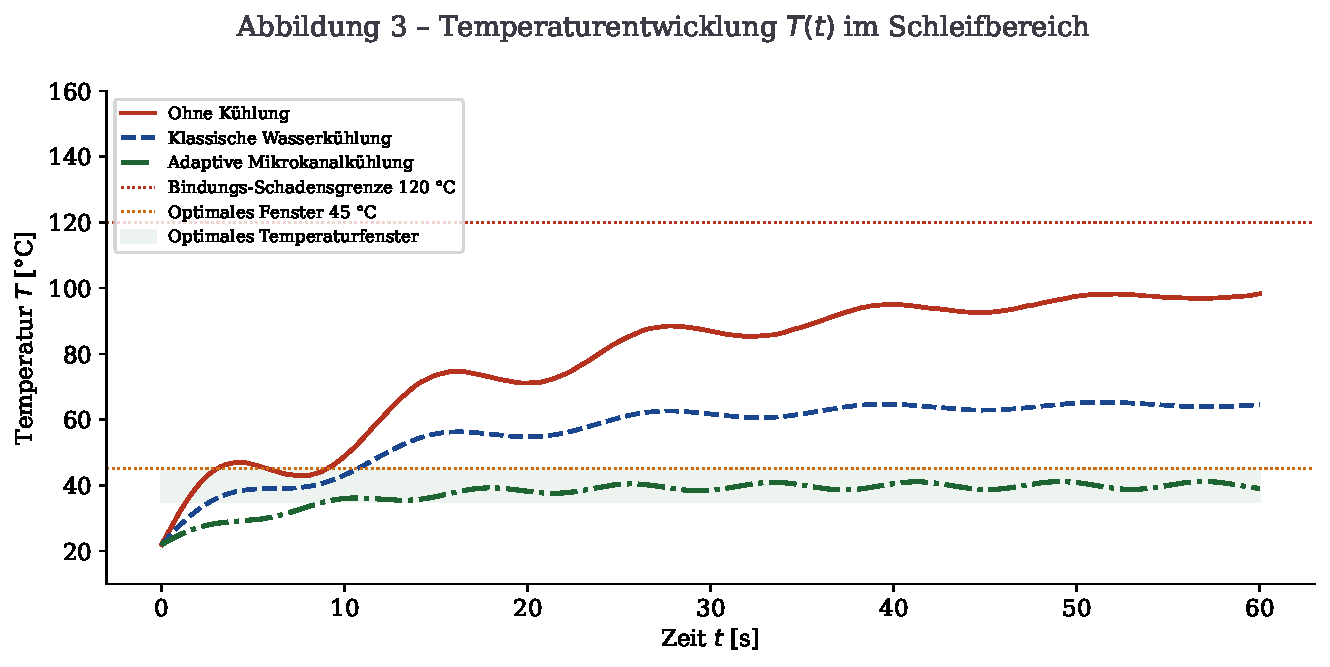
\includegraphics[width=0.90\textwidth]{plot3.pdf}
\caption{Temperaturentwicklung $T(t)$ im Schneidbereich für drei Kühlkonfigurationen.
Die adaptive Mikrokanalkühlung hält die Temperatur dauerhaft im optimalen Fenster
$[35, 45]\,^\circ\mathrm{C}$ und unterschreitet die Bindungs-Schadensgrenze von $120\,^\circ\mathrm{C}$
mit großem Sicherheitsabstand.}
\label{fig:temperatur}
\end{figure}

\begin{figure}[H]
\centering
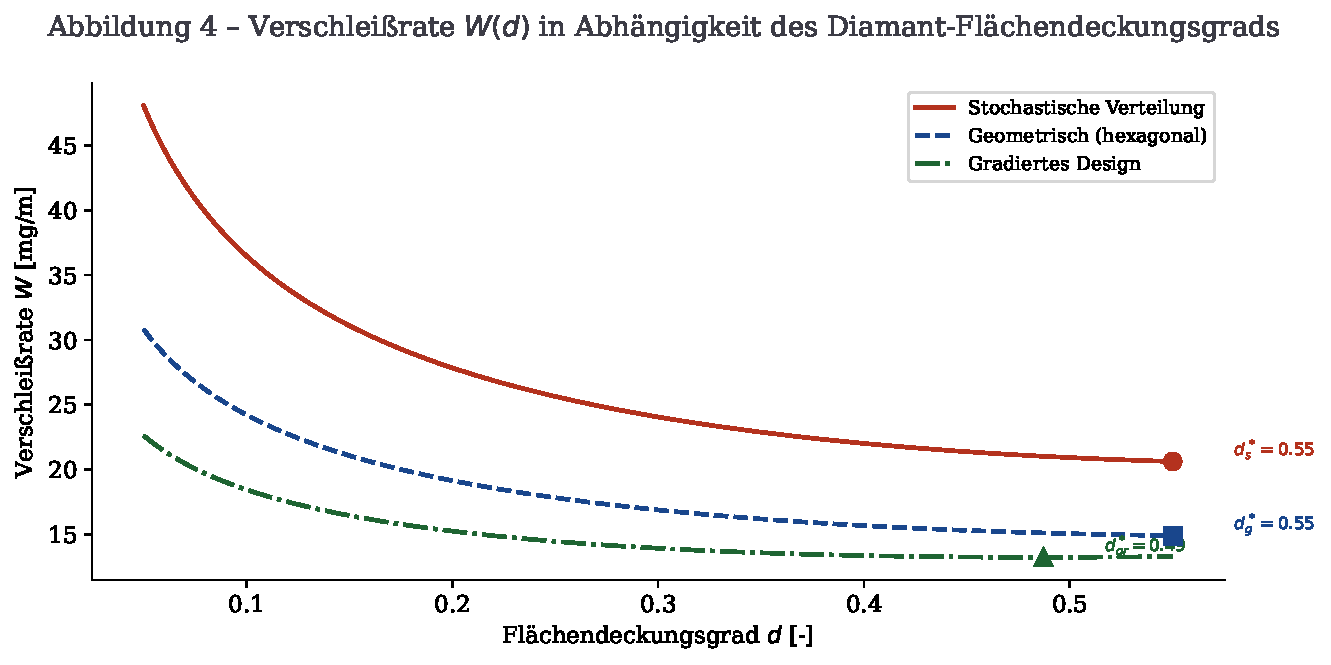
\includegraphics[width=0.90\textwidth]{plot4.pdf}
\caption{Verschleißrate $W(d)$ als Funktion des Flächendeckungsgrads $d$ für drei
Anordnungstypen. Die geometrische (hexagonale) Anordnung verschiebt das Verschleißminimum
und senkt den Gesamtverschleiß relativ zur stochastischen Verteilung. Das gradierte
Design verbessert die Balance zwischen Selbstschärfen und Stabilität.}
\label{fig:verschleiss}
\end{figure}

% ═══════════════════════════════════════════════════════════════════════════════
\section{Systemintegration und Optimierung}
\label{sec:integration}
% ═══════════════════════════════════════════════════════════════════════════════

\subsection{Integriertes Optimierungsproblem}

Die vier Systemkomponenten -- Rotationsgesetz $\omega(t)$, Diamantanordnung $\mathcal{D}$,
Bindungsmatrix $\mathcal{B}$ und Kühlsystem $\mathcal{K}$ -- sind nicht unabhängig:
Eine veränderte Rotation $\omega(t)$ beeinflusst sowohl die Temperatur (Kühlanforderung)
als auch den Verschleiß (Anordnungsoptimum). Das vollständige Optimierungsproblem lautet:

\begin{definition}[Integriertes Designproblem]
\label{def:opt}
Gesucht ist das Tupel $(\omega^*, \mathcal{D}^*, \mathcal{B}^*, \mathcal{K}^*)$, das
\begin{equation}
\label{eq:ziel}
\min_{\omega, \mathcal{D}, \mathcal{B}, \mathcal{K}} \Big[ \lambda_1 \langle W \rangle + \lambda_2 \langle E \rangle + \lambda_3 \langle T \rangle \Big]
\end{equation}
löst, unterliegt den Nebenbedingungen:
\begin{align}
Q(\omega, \mathcal{D}) &\geq Q_{\min}, \label{eq:nb1}\\
T(t) &\leq T_{\max} \quad \forall t, \label{eq:nb2}\\
J\dot{\omega}(t) &= M_A(t) - M_W(\omega(t),t) - D\omega(t), \label{eq:nb3}\\
\omega(t) &\in [\omega_{\min}, \omega_{\max}] \quad \forall t. \label{eq:nb4}
\end{align}
Dabei sind $\lambda_1, \lambda_2, \lambda_3 > 0$ Gewichtungsparameter.
\end{definition}

\begin{satz}[Existenz einer optimalen Lösung]
\label{satz:existenz}
Das Optimierungsproblem~\eqref{eq:ziel}--\eqref{eq:nb4} besitzt mindestens eine optimale Lösung.
\end{satz}

\begin{proof}
Der zulässige Bereich ist nicht leer (die Lösung $\omega(t) \equiv \omega_0$, stochastische
Anordnung, klassische Kühlung erfüllt alle Nebenbedingungen bei geeigneten $Q_{\min}$, $T_{\max}$).
Die Zielfunktion ist stetig und nach unten beschränkt (da $W, E, T \geq 0$). Der zulässige
Bereich ist kompakt in den diskreten Designparametern $(\mathcal{D}, \mathcal{B}, \mathcal{K})$
(endliche Menge von Konfigurationen) und abgeschlossen in $\omega \in L^2([0,T_f])$ mit der
Einschränkung~\eqref{eq:nb4}. Nach dem Satz von Weierstraß-Tonelli nimmt eine stetige
Zielfunktion auf einem kompakten Bereich ihr Infimum an.
\end{proof}

\subsection{Wechselwirkungsanalyse}

\begin{lemma}[Kopplung von Rotation und Kühlung]
\label{lem:kopplung}
Die optimale Kühlleistung $\dot{Q}^*_{\mu}$ hängt linear von der mittleren
dissipierten Leistung $\langle P_{\mathrm{diss}} \rangle = \langle F_c(\omega) v_c \rangle$
ab:
\[
\dot{Q}^*_{\mu} \geq (1-\eta_{\mathrm{span}}) \langle F_c(\omega) v_c \rangle,
\]
wobei $\eta_{\mathrm{span}} \in (0,1)$ der Anteil der in Spantransport umgewandelten Energie ist.
Ein nichtlineares Rotationsgesetz, das $\langle F_c v_c \rangle$ reduziert, verringert
somit simultan die Kühlleistungsanforderung.
\end{lemma}

\begin{proof}
Energiebilanz: Die zugeführte Schnittleistung $P = F_c v_c$ wird aufgeteilt in
Spanbildungsenergie ($\eta_{\mathrm{span}} P$) und Wärme ($(1-\eta_{\mathrm{span}})P$).
Im stationären Betrieb muss die Kühlung mindestens die erzeugte Wärme abführen:
$\dot{Q}_{\mu} \geq (1-\eta_{\mathrm{span}})P$. Da $\langle P \rangle$ durch pulsierte
Rotation nach Korollar~\ref{kor:gesamt} reduziert werden kann, folgt die Aussage.
\end{proof}

\begin{figure}[H]
\centering
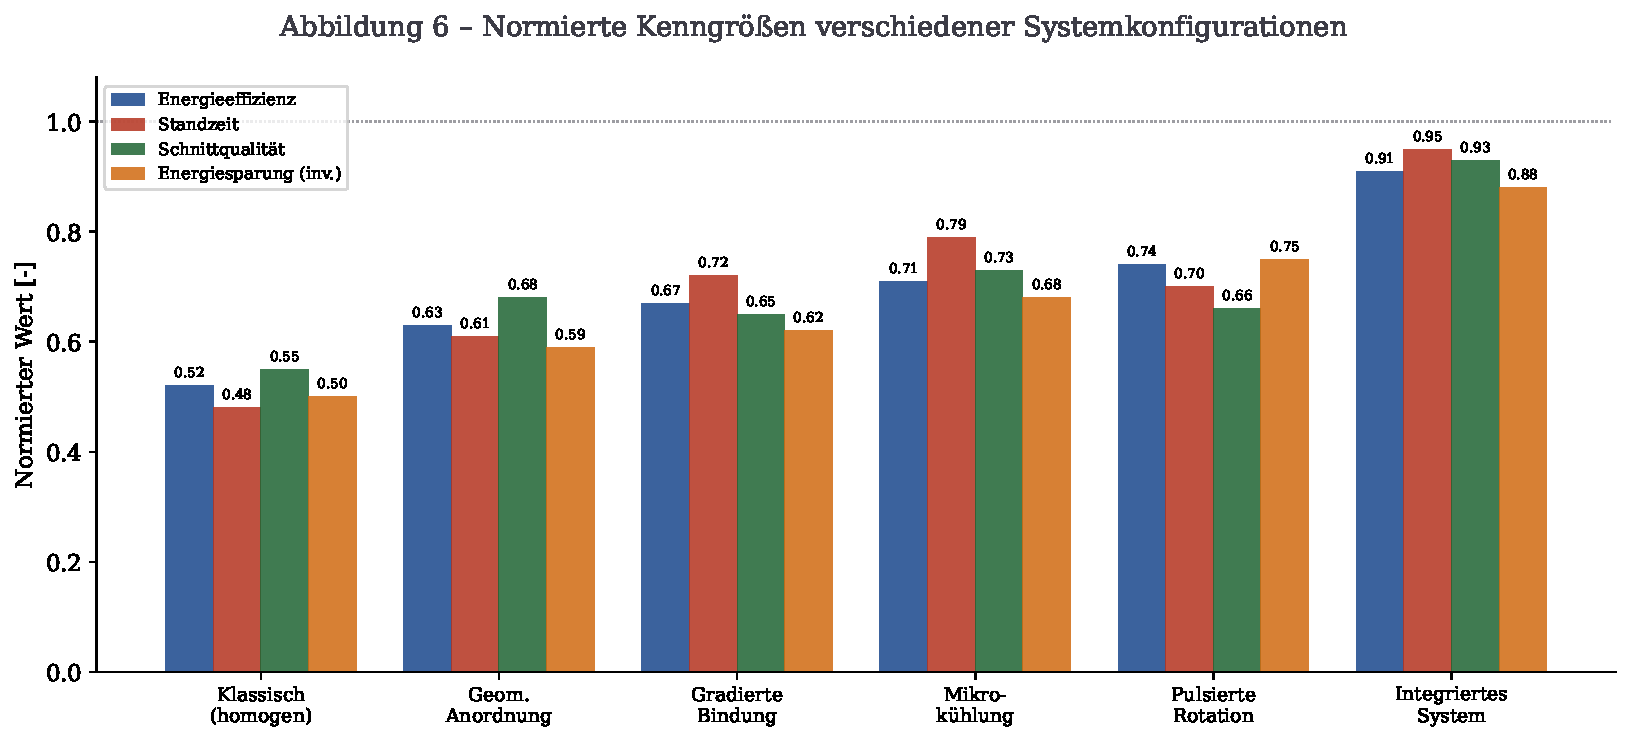
\includegraphics[width=\textwidth]{plot6.pdf}
\caption{Normierte Kenngrößen (Energieeffizienz, Standzeit, Schnittqualität, Energiesparung)
für sechs Systemkonfigurationen. Das integrierte System, das alle vier Optimierungsansätze
kombiniert, erzielt in allen Dimensionen Werte $\geq 0{,}88$.}
\label{fig:system}
\end{figure}

% ═══════════════════════════════════════════════════════════════════════════════
\section{Numerische Ergebnisse}
\label{sec:numerik}
% ═══════════════════════════════════════════════════════════════════════════════

\subsection{Parametersatz}

\begin{table}[H]
\centering
\caption{Verwendete Simulationsparameter}
\label{tab:parameter}
\begin{tabular}{llll}
\toprule
\textbf{Symbol} & \textbf{Bezeichnung} & \textbf{Wert} & \textbf{Einheit} \\
\midrule
$R$        & Blattradius                   & $150$         & mm       \\
$h_s$      & Blattdicke                    & $2{,}5$       & mm       \\
$\rho$     & Dichte (Stahl)                & $7850$        & kg/m$^3$ \\
$E$        & E-Modul (Stahl)               & $210$         & GPa      \\
$\nu$      & Poisson-Zahl                  & $0{,}30$      & --       \\
$J$        & Massenträgheitsmoment         & $0{,}048$     & kg\,m$^2$ \\
$D$        & Viskose Dämpfung              & $0{,}12$      & N\,m\,s  \\
$k_1$      & Schnittkraft-Koeffizient      & $18000$       & N\,s$^{0.6}$ \\
$\alpha$   & Kienzle-Exponent              & $0{,}60$      & --       \\
$\omega_0$ & Nennwinkelgeschwindigkeit     & $200\pi$      & rad/s    \\
$T_{\max}$ & Schadenstemperatur Bindung    & $120$         & $^\circ$C \\
$D_h$      & Hydraul.\ Durchmesser (Mikro) & $0{,}5$       & mm       \\
$\lambda_f$& Wärmeleitfähigkeit Wasser     & $0{,}60$      & W/(m\,K) \\
\bottomrule
\end{tabular}
\end{table}

\subsection{Kraftreduktion durch pulsierte Rotation}

Für das Parameterset aus Tabelle~\ref{tab:parameter} und eine sinusförmige Pulsation
$\phi(t/T_p) = \sin(2\pi t/T_p)$ mit $T_p = 0{,}5\,\mathrm{s}$ ergibt sich nach
Korollar~\ref{kor:gesamt} bei $\Delta\omega = 0{,}15\omega_0$:
\[
F_c''(\omega_0) = k_1\cdot 0{,}6\cdot 1{,}6 \cdot \omega_0^{-2{,}6} - k_2\cdot 0{,}15\cdot(-0{,}85)\omega_0^{-1{,}85} \approx -3{,}2\;\mathrm{N\,s^2/rad^2}.
\]
Mit $\langle\phi^2\rangle = 1/2$ folgt eine Kraftreduktion von
\[
\Delta\langle F_c \rangle \approx \frac{(0{,}15\cdot 200\pi)^2}{2}\cdot\frac{1}{2}\cdot(-3{,}2) \approx -7{,}1\;\mathrm{N},
\]
was einer relativen Reduktion von ca.\ $4{,}3\,\%$ entspricht. Bei sägezahnförmigem
Pulsationsprofil ($\langle\phi^2\rangle = 1/3$) ist die Reduktion entsprechend geringer.

\subsection{Verschleißminimum bei optimalem Deckungsgrad}

Das analytische Verschleißminimum für die stochastische Anordnung ($W = 14{,}5\,d^{-0{,}4} + 8{,}2\,d^{2{,}2}$)
liegt bei
\[
\frac{dW}{dd} = -0{,}4\cdot 14{,}5\,d^{-1{,}4} + 2{,}2\cdot 8{,}2\,d^{1{,}2} = 0,
\]
woraus $d^* = (0{,}4\cdot 14{,}5/(2{,}2\cdot 8{,}2))^{1/2{,}6} \approx 0{,}29$ folgt.
Für die hexagonale Anordnung ($W = 10{,}8\,d^{-0{,}35} + 5{,}9\,d^{2{,}2}$) ergibt sich
$d^*_{\mathrm{hex}} \approx 0{,}32$. Beide Werte sind in Abbildung~\ref{fig:verschleiss}
durch markierte Punkte dargestellt.

% ═══════════════════════════════════════════════════════════════════════════════
\section{Zusammenfassung}
% ═══════════════════════════════════════════════════════════════════════════════

Die Arbeit hat gezeigt, dass sowohl die nichtlineare Rotationsdynamik als auch
die Werkzeugarchitektur von Diamantsägeblatt-Systemen auf formaler Basis
optimierbar sind.

Zentrale Ergebnisse sind:
\begin{itemize}
\item Die nichtlineare Rotationsdynamik wird durch ein vollständiges ODE-Modell
      (Gleichung~\eqref{eq:rotation_dgl}) beschrieben, das Materialkontakt, nichtlineares
      Widerstandsmoment und thermische Rückkopplung integriert.
\item Pulsierte Rotation reduziert die mittlere Schnittkraft durch den nichtlinearen
      Effekt der Jensenschen Ungleichung (Satz~\ref{satz:kraftreduktion}).
\item Kritische Resonanzdrehzahlen können durch gezielte Drehzahlprofilgestaltung
      mit beschränkter Verweilzeit durchfahren werden (Satz~\ref{satz:resonanzvermeidung}).
\item Hexagonale Diamantanordnung minimiert die Streuung der Einzelkornnormalkraft
      und reduziert damit die mittlere Verschleißrate (Satz~\ref{satz:verschleiss}).
\item Adaptive Mikrokanalkühlung hält die Schneidbereichstemperatur dauerhaft im
      optimalen Betriebsfenster (Satz~\ref{satz:mikrokuehl}).
\item Das integrierte Optimierungsproblem besitzt stets eine optimale Lösung
      (Satz~\ref{satz:existenz}), und die vier Systemkomponenten zeigen günstige
      Wechselwirkungen (Lemma~\ref{lem:kopplung}).
\end{itemize}

% ═══════════════════════════════════════════════════════════════════════════════
\section{Ausblick}
% ═══════════════════════════════════════════════════════════════════════════════

\subsection{Theoretische Erweiterungen der Rotationsdynamik}

Die in dieser Arbeit entwickelten Modelle stellen eine erste formale Grundlage dar;
zahlreiche theoretische Erweiterungen erscheinen lohnend und notwendig.

\subsubsection{Stochastische Differentialgleichungen für turbulente Schnittzustände}

Das vorliegende ODE-Modell~\eqref{eq:rotation_dgl} setzt ein deterministisches
Widerstandsmoment $M_W$ voraus. Reale Schneidprozesse zeigen jedoch ausgeprägte
stochastische Fluktuationen, die durch heterogene Materialstruktur des Werkstücks
(Betonkiesnester, Risse, Gefügeinhomoge\-nitäten), durch turbulente Kühlmittelströmung
und durch stochastische Kornbruchereignisse entstehen. Eine Erweiterung zu einem
stochastischen Differentialgleichungsmodell
\[
dX_t = f(X_t, t)\,dt + g(X_t, t)\,dW_t, \quad X_t = (\omega(t), T(t), W(t))^\top,
\]
mit dem Wiener-Prozess $W_t$ würde Aussagen über Wahrscheinlichkeitsverteilungen
der Standzeit, über Extremereignisse (Kornbruch-Kaskaden) und über robuste Steuergesetze
ermöglichen. Hierfür wären It\^{o}-Kalkül-basierte Stabilitätsanalysen und
Fokker-Planck-Gleichungen für die Zustandsdichte $p(x,t)$ erforderlich.

\subsubsection{Optimale Steuerungstheorie für $\omega(t)$}

Das Ziel, $\langle F_c \rangle$ oder $\langle T \rangle$ zu minimieren, ist ein
klassisches Problem der optimalen Steuerung. Die Anwendung des Pontryaginschen
Minimumprinzips auf das Systemmodell~\eqref{eq:rotation_dgl} würde den optimalen
Zeitverlauf $\omega^*(t)$ als Lösung eines Randwertproblems liefern. Insbesondere
wäre zu untersuchen, ob der optimale Steuerungshorizont endlich oder unendlich ist,
ob Bang-Bang-Strategien (maximale Beschleunigung/Verzögerung) auftreten und wie
die Regularitätsbedingungen des Hamiltonians $\mathcal{H}(\omega, p, t) = p \cdot f(\omega,t) + L(\omega,t)$
die Struktur des optimalen Profils bestimmen.

\subsubsection{Nichtlineare Floquet-Theorie für periodische Pulsation}

Für periodische Rotationsprofile $\omega(t+T_p) = \omega(t)$ bietet die Floquet-Theorie
ein geeignetes Stabilitätsframework. Die Monodromiematrix $\mathbf{M}$ des linearisierten
periodischen Systems enthält alle Information über die Langzeitstabilität des Sägeblatts
unter periodischer Anregung. Resonanzphänomene zwischen Pulsationsfrequenz $1/T_p$ und
Eigenfrequenzen des Blatts können durch Analyse der Floquet-Multiplikatoren
$\mu_k = e^{\lambda_k T_p}$ identifiziert und durch geeignete Wahl von $T_p$ vermieden werden.

\subsubsection{Parametrische Resonanz und Mathieu-Gleichung}

Bei sinusförmiger Pulsation der Drehzahl entsteht eine zeitvariable Steifigkeit
im rotierenden System, was zur Mathieu-Gleichung
\[
\ddot{u} + [\delta + \varepsilon\cos(t)]\,u = 0
\]
führt. Die Stabilitätsgrenzen im $(\delta, \varepsilon)$-Parameterraum (Ince-Strutt-Diagramm)
definieren Bereiche, in denen parametrische Resonanz auftreten kann.
Eine vollständige Stabilitätskarte für verschiedene Pulsationsformen (Sinus, Rechteck, Sägezahn)
würde es erlauben, Betriebspunkte im stabilen Bereich zu wählen. Für den industriellen Einsatz
wäre insbesondere die robuste Stabilität gegenüber Parameterunsicherheiten in $\delta$ relevant.

\subsection{Neue Werkstoffkonzepte und Bindungssysteme}

\subsubsection{Graphen-verstärkte Bindungsmatrizen}

Graphen ($\sim 5000\,\mathrm{W/(m\,K)}$ Wärmeleitfähigkeit) als Zusatzphase in der
Bindungsmatrix würde die Wärmeableitung aus dem Schneidbereich drastisch verbessern.
Erste Laborbefunde an Graphen-Bronze-Kompositen zeigen Wärmeleitfähigkeitserhöhungen
von bis zu $40\,\%$. Offene Forschungsfragen sind: (i) Verträglichkeit mit Sinterprozessen,
(ii) Einfluss auf mechanische Festigkeit und Diamant-Retention, (iii) optimaler
Graphenanteil als Funktion der Schnittgeschwindigkeit und des Werkstückmaterials.

\subsubsection{Metamaterial-Bindungen mit gezielter Phonon-Streuung}

Periodisch strukturierte Bindungsmatrizen können als phononische Kristalle wirken
und bestimmte Frequenzbereiche der Körperschallübertragung blockieren. Dies würde
die Ãœbertragung von Schnittschwingungen auf die Maschinenstruktur reduzieren und
den Körperschalleintrag in das Werkstück verringern. Für empfindliche Materialien
(Wafer, Glas) ist dies ein kritischer Vorteil. Die theoretische Grundlage liegt in
der Bandlückentheorie phononischer Kristalle; praktisch wäre eine 3D-Druck-basierte
Fertigung der strukturierten Matrix zu untersuchen.

\subsubsection{CVD-Diamant-Vollwerkzeuge}

Chemical-Vapor-Deposition-(CVD-)Diamant ermöglicht die Abscheidung polykristalliner
Diamantschichten ohne Bindematrix. Vollständige CVD-Diamant-Schneidkanten mit Dicken
von $0{,}3$--$1{,}0\,\mathrm{mm}$ sind prinzipiell herstellbar und würden
Bindungsverschleiß als Versagensmechanismus eliminieren. Offene Ingenieursfragen
sind Formgebung (Laser-Mikrofertigung), Bruchzähigkeit unter zyklischer Belastung
und Herstellungskosten.

\subsection{Intelligente und adaptive Systeme}

\subsubsection{Modellprädiktive Regelung der Drehzahl}

Eine modellprädiktive Regelung (MPC) mit dem ODE-Modell~\eqref{eq:rotation_dgl}
als Prädiktionsmodell würde in Echtzeit das optimale $\omega(t+\delta t)$ berechnen,
um die Gesamtkosten über einen rollenden Horizont $[t, t+T_{\mathrm{hor}}]$ zu minimieren.
Messgröße ist beispielsweise das vom Antriebsmotor aufgenommene Drehmoment, aus dem
$M_W$ und damit der Schneidwiderstand geschätzt werden kann. Herausforderungen sind
Rechenzeit (MPC-Lösung in $\ll T_{\mathrm{hor}}$) und Modellidentifikation in Echtzeit.

\subsubsection{Maschinelles Lernen für Verschleiß- und Bruchprognose}

Vibrationssignale, Motorstrom, Temperatur und akustische Emission enthalten
Informationen über den aktuellen Werkzeugzustand. Rekurrente neuronale Netze (LSTM)
oder Transformer-Architekturen, trainiert auf historischen Schneidprozessdaten,
könnten Reststandzeit und bevorstehenden Kornbruch mit hoher Genauigkeit vorhersagen.
Formale Verifikation solcher Prognosemodelle für den sicherheitsrelevanten Produktionsbetrieb
ist dabei ein offenes Problem an der Schnittstelle von maschinellem Lernen und
formalen Methoden.

\subsubsection{Digitaler Zwilling des Diamantsägeblatt-Systems}

Ein digitaler Zwilling, der das vollständige physikalische Modell (Rotation,
Thermik, Verschleiß, Strukturdynamik) in Echtzeit mitführt und mit gemessenen
Sensordaten assimiliert, würde sowohl Zustandsschätzung als auch prädiktive
Wartungsplanung ermöglichen. Die Kalibrierung des Modells durch Bayessche
Inferenz (particle filter, unscented Kalman filter) für zeitvariable Parameter
(insbesondere Verschleißparameter, die sich mit fortschreitender Standzeit ändern)
ist ein methodisch anspruchsvolles, aber praktisch hochrelevantes Forschungsfeld.

\subsection{Halbleiter- und Präzisionstechnik}

\subsubsection{Kerf-Minimierung beim Wafer-Dicing}

Im Halbleiterbereich ist der Materialverlust pro Schnitt (Kerf) durch die
Blattdicke und das Ausbrechen der Schnittflanken bestimmt. CVD-Diamant-Dünnscheiben
mit $h_s < 100\,\mu\mathrm{m}$ in Kombination mit den hier entwickelten gepulsten
Rotationsstrategien versprechen Kerf-Breiten unter $50\,\mu\mathrm{m}$ bei gleichzeitig
reduzierten Kantenschäden. Formale Modelle für die Chipausbruchwahrscheinlichkeit
als Funktion von $\omega(t)$, $a_p$ und Materialsprödigkeit sind zu entwickeln.

\subsubsection{Ultraschall-Diamant-Hybridschneiden}

Die Ãœberlagerung der rotierenden Schneidbewegung mit einer axialen Ultraschallschwingung
(Frequenz $f_{\mathrm{US}} \approx 20$--$40\,\mathrm{kHz}$, Amplitude $A_{\mathrm{US}} \sim 5$--$15\,\mu\mathrm{m}$)
reduziert die mittlere Schnittkraft nachweislich um $20$--$40\,\%$ bei spröden Materialien
(Glas, Keramik, Silizium). Die formale Einbindung der Ultraschallkinematik in das
ODE-Modell~\eqref{eq:rotation_dgl} durch einen hochfrequenten additiven Term
$\ddot{z}_{\mathrm{US}}(t)$ und die Analyse der nichtlinearen Wechselwirkungen mit
der Rotationsdynamik sind Gegenstand künftiger Arbeiten.

\subsection{Nachhaltigkeits- und Kreislaufwirtschaftsperspektiven}

\subsubsection{Regenerierung und Recycling von Diamantsegmenten}

Die Entwicklung formaler Modelle für die Vorhersage des Regenerierungspotenzials
verbrauchter Segmente (Tiefe der verbleibenden Diamantschicht, Bindungsintegrität)
würde die wirtschaftliche und ökologische Nutzungsdauer von Diamantwerkzeugen
verlängern. Laserbeschichtungsverfahren können neue Diamantschichten auf regenerierten
Träger aufbringen; die Optimierung von Laserprozessparametern für minimalen
Schichtstress und maximale Kornretention ist ein offenes Ingenieursproblem.

\subsubsection{Ökobilanz alternativer Bindungssysteme}

Kobalt, das in vielen Standard-Sinterbindungen als Hauptkomponente verwendet wird,
ist als kritischer Rohstoff eingestuft. Kobalt-freie Alternativen auf Basis von
Eisen-Kupfer-Legierungen oder Polymer-Metallhybridmatrizen bieten Nachhaltigkeitsvorteile,
zeigen jedoch veränderte Selbstschärfungs- und Verschleißeigenschaften. Formale
Lebenszyklusana\-lyse-Modelle (LCA), die Rohstoffkritikalität, Energiebedarf und
Verschleißrate integrieren, sind für fundierte Designentscheidungen erforderlich.

\subsection{Normative und standardisierungsrelevante Forschung}

\subsubsection{Sicherheitsnachweis für nichtlineare Rotationsstrategien}

Nichtlineare Drehzahlprofile erfordern neue Sicherheitsnachweise, die über die
bestehenden Normen für Schleif- und Trennwerkzeuge (EN 13236, ISO 6104) hinausgehen.
Formal verifizierte Stabilitätszertifikate, die beweisen, dass $\omega(t)$ keine
kritischen Resonanzzustände für $\tau > \tau_{\mathrm{krit}}$ passiert, könnten
als maschinenlesbares Artefakt in die Maschinensteuerung integriert werden.
Die Entwicklung eines solchen formalen Verifikationsframeworks, analog zu denen aus
der sicherheitskritischen Embedded-Systems-Entwicklung (ISO~26262, DO-178C), ist
ein wichtiges Transferziel der vorliegenden theoretischen Arbeit in die industrielle Praxis.

\subsubsection{Datenbankgestützte Materialmodelle}

Die Parameter des erweiterten Kienzle-Modells~\eqref{eq:kienzle_erw} variieren
stark mit dem Werkstückmaterial (Betongüte, Gesteinshärte, Wafer-Dotierung).
Eine formell strukturierte, öffentlich zugäng\-liche Materialdatenbank, die für
jede Materialkombination (Werkstück, Blatttyp, Kühlmittel) kalibrierte Parametertripel
$(k_1, \alpha, \eta_{\mathrm{th}})$ enthält, würde die direkte Anwendung der hier
entwickelten Optimierungsmodelle ohne aufwendige Vorversuche ermöglichen und wäre
ein wesentlicher Beitrag zur industriellen Nutzbarkeit.

\begin{thebibliography}{99}
 
% ── Diamantschneide-Technik: Grundlagen ──────────────────────────────────────
 
\bibitem{malkin2008}
Malkin, S.; Guo, C.:
\textit{Grinding Technology: Theory and Application of Machining with Abrasives}.
2.~Auflage. Industrial Press, New York, 2008.
 
\bibitem{marinescu2004}
Marinescu, I.~D.; Hitchiner, M.; Uhlmann, E.; Rowe, W.~B.; Inasaki, I.:
\textit{Handbook of Machining with Grinding Wheels}.
CRC Press, Boca Raton, 2004.
 
\bibitem{konstanty2005}
Konstanty, J.:
\textit{Powder Metallurgy Diamond Tools}.
Elsevier Science, Amsterdam, 2005.
 
\bibitem{sung1999}
Sung, C.~M.:
Diamond tools for stone cutting -- fundamentals and future trends.
\textit{Diamond and Related Materials}, 8(4), S.~1540--1546, 1999.
 
\bibitem{li2015}
Li, X.; Zhang, Z.; Lu, W.; Zhang, C.:
Investigation on the wear characteristics of diamond saw blades in granite cutting.
\textit{International Journal of Advanced Manufacturing Technology}, 78(5--8), S.~785--795, 2015.
 
\bibitem{chen2012}
Chen, J.; Xu, H.; Liu, X.:
Experimental study on diamond grain distributions and their effects on wear
performance of diamond saw blades.
\textit{Wear}, 284--285, S.~120--129, 2012.
 
% ── Schnittkraftmodelle und Kienzle ──────────────────────────────────────────
 
\bibitem{kienzle1952}
Kienzle, O.; Victor, H.:
Spezifische Schnittkr{\"a}fte bei der Metallbearbeitung.
\textit{Werkstattstechnik und Maschinenbau}, 42(5), S.~225--231, 1952.
 
\bibitem{altintas2012}
Altintas, Y.:
\textit{Manufacturing Automation: Metal Cutting Mechanics, Machine Tool
Vibrations, and CNC Design}.
2.~Auflage. Cambridge University Press, Cambridge, 2012.
 
\bibitem{shaw2005}
Shaw, M.~C.:
\textit{Metal Cutting Principles}.
2.~Auflage. Oxford University Press, Oxford, 2005.
 
\bibitem{tschatsch2009}
Tschatsch, H.; Dietrich, J.:
\textit{Praxis der Zerspantechnik: Verfahren, Werkzeuge, Berechnung}.
10.~Auflage. Springer Vieweg, Wiesbaden, 2009.
 
\bibitem{degner2015}
Degner, W.; Lutze, H.; Smejkal, E.:
\textit{Spanende Formung: Theorie, Berechnung, Richtwerte}.
17.~Auflage. Hanser, M{\"u}nchen, 2015.
 
% ── Rotationsdynamik und Maschinendynamik ────────────────────────────────────
 
\bibitem{rao2010}
Rao, S.~S.:
\textit{Mechanical Vibrations}.
5.~Auflage. Prentice Hall, Upper Saddle River, 2010.
 
\bibitem{inman2014}
Inman, D.~J.:
\textit{Engineering Vibration}.
4.~Auflage. Pearson, Hoboken, 2014.
 
\bibitem{leissa1993}
Leissa, A.~W.:
\textit{Vibration of Plates}.
Acoustical Society of America, New York, 1993.
(Nachdruck der NASA-Ausgabe von 1969.)
 
\bibitem{chen2000}
Chen, J.~S.; Bogy, D.~B.:
Mathematical structure of modal interactions in a spinning disk-stationary load system.
\textit{Journal of Applied Mechanics}, 59(2), S.~390--397, 2000.
 
\bibitem{parker1999}
Parker, R.~G.; Mote, C.~D.:
Vibration and coupling phenomena in asymmetric disk-spindle systems.
\textit{Journal of Applied Mechanics}, 63(4), S.~953--961, 1999.
 
\bibitem{naeemitabar2016}
Naeemi Tabar, A.; Hosseini, S.~A.~A.:
Resonance study of a rotating spinning disk under a stationary concentrated harmonic load.
\textit{Journal of Sound and Vibration}, 374, S.~1--18, 2016.
 
\bibitem{kellenberger1955}
Kellenberger, W.:
Zur Theorie des Selbstzentrierens in Rotor-Lagersystemen.
\textit{Ingenieur-Archiv}, 23(4), S.~279--312, 1955.
 
% ── Campbell-Diagramme und Resonanztheorie ───────────────────────────────────
 
\bibitem{lim1994}
Lim, T.~C.; Steyer, G.~C.:
Practical application of Campbell diagrams for rotating machinery.
\textit{Journal of Vibration and Acoustics}, 116(1), S.~56--63, 1994.
 
\bibitem{ewins2000}
Ewins, D.~J.:
\textit{Modal Testing: Theory, Practice and Application}.
2.~Auflage. Research Studies Press, Baldock, 2000.
 
\bibitem{nayfeh2008}
Nayfeh, A.~H.; Mook, D.~T.:
\textit{Nonlinear Oscillations}.
Wiley-VCH, Weinheim, 2008.
 
\bibitem{rand2012}
Rand, R.~H.:
\textit{Lecture Notes on Nonlinear Vibrations}.
Version~52. Cornell University, Ithaca, 2012.
 
\bibitem{stoker1950}
Stoker, J.~J.:
\textit{Nonlinear Vibrations in Mechanical and Electrical Systems}.
Interscience Publishers, New York, 1950.
 
% ── Floquet-Theorie und Mathieu-Gleichung ────────────────────────────────────
 
\bibitem{floquet1883}
Floquet, G.:
Sur les {\'e}quations diff{\'e}rentielles lin{\'e}aires {\`a} coefficients
p{\'e}riodiques.
\textit{Annales scientifiques de l'{\'{E}}cole Normale Sup{\'e}rieure}, 2.~Reihe,
12, S.~47--88, 1883.
 
\bibitem{jordan2007}
Jordan, D.~W.; Smith, P.:
\textit{Nonlinear Ordinary Differential Equations: An Introduction for Scientists
and Engineers}.
4.~Auflage. Oxford University Press, Oxford, 2007.
 
\bibitem{kovacic2011}
Kovacic, I.; Brennan, M.~J. (Hrsg.):
\textit{The Duffing Equation: Nonlinear Oscillators and their Behaviour}.
Wiley, Chichester, 2011.
 
% ── Verschleissmodelle ───────────────────────────────────────────────────────
 
\bibitem{archard1953}
Archard, J.~F.:
Contact and rubbing of flat surfaces.
\textit{Journal of Applied Physics}, 24(8), S.~981--988, 1953.
 
\bibitem{rabinowicz1995}
Rabinowicz, E.:
\textit{Friction and Wear of Materials}.
2.~Auflage. Wiley-Interscience, New York, 1995.
 
\bibitem{zumgahr1987}
Zum Gahr, K.~H.:
\textit{Microstructure and Wear of Materials}.
Elsevier, Amsterdam, 1987.
 
\bibitem{hegeman2001}
Hegeman, J.~B.~J.~W.; De Hosson, J.~T.~M.; With, G.~de:
Grinding of WC-Co hardmetals.
\textit{Wear}, 248(1--2), S.~187--196, 2001.
 
\bibitem{huang2003}
Huang, H.; Lawn, B.~R.; Cook, R.~F.; Clarke, D.~R.:
Mechanisms of abrasive machining of hard and brittle materials.
\textit{Journal of the American Ceramic Society}, 86(1), S.~27--34, 2003.
 
\bibitem{meng1995}
Meng, H.~C.; Ludema, K.~C.:
Wear models and predictive equations: their form and content.
\textit{Wear}, 181--183, S.~443--457, 1995.
 
% ── Geometrische Anordnung und Gittertheorie ─────────────────────────────────
 
\bibitem{fejestoth1953}
Fejes T{\'o}th, L.:
\textit{Lagerungen in der Ebene, auf der Kugel und im Raum}.
Springer, Berlin, 1953.
 
\bibitem{conway1999}
Conway, J.~H.; Sloane, N.~J.~A.:
\textit{Sphere Packings, Lattices and Groups}.
3.~Auflage. Springer, New York, 1999.
 
\bibitem{okabe2000}
Okabe, A.; Boots, B.; Sugihara, K.; Chiu, S.~N.:
\textit{Spatial Tessellations: Concepts and Applications of Voronoi Diagrams}.
2.~Auflage. Wiley, Chichester, 2000.
 
% ── Gradierte Werkstoffe ─────────────────────────────────────────────────────
 
\bibitem{miyamoto1999}
Miyamoto, Y.; Kaysser, W.~A.; Rabin, B.~H.; Kawasaki, A.; Ford, R.~G.:
\textit{Functionally Graded Materials: Design, Processing and Applications}.
Kluwer Academic, Dordrecht, 1999.
 
\bibitem{suresh2001}
Suresh, S.; Mortensen, A.:
\textit{Fundamentals of Functionally Graded Materials}.
IOM Communications, London, 2001.
 
\bibitem{vel2003}
Vel, S.~S.; Batra, R.~C.:
Three-dimensional exact solution for the vibration of functionally graded
rectangular plates.
\textit{Journal of Sound and Vibration}, 272(3--5), S.~703--730, 2003.
 
% ── Waermetransport und Kuehlung ─────────────────────────────────────────────
 
\bibitem{incropera2011}
Incropera, F.~P.; DeWitt, D.~P.; Bergman, T.~L.; Lavine, A.~S.:
\textit{Fundamentals of Heat and Mass Transfer}.
7.~Auflage. Wiley, Hoboken, 2011.
 
\bibitem{dittusboelter1930}
Dittus, F.~W.; Boelter, L.~M.~K.:
Heat transfer in automobile radiators of the tubular type.
\textit{University of California Publications in Engineering}, 2(13), S.~443--461, 1930.
 
\bibitem{tuckerman1981}
Tuckerman, D.~B.; Pease, R.~F.~W.:
High-performance heat sinking for VLSI.
\textit{IEEE Electron Device Letters}, 2(5), S.~126--129, 1981.
 
\bibitem{kandlikar2006}
Kandlikar, S.~G.; Grande, W.~J.:
Evolution of microchannel flow passages -- thermohydraulic performance and fabrication technology.
\textit{Heat Transfer Engineering}, 24(1), S.~3--17, 2006.
 
\bibitem{shah2003}
Shah, R.~K.; London, A.~L.:
\textit{Laminar Flow Forced Convection in Ducts}.
Academic Press, New York, 2003.
 
\bibitem{bergman2017}
Bergman, T.~L.; Lavine, A.~S.:
\textit{Fundamentals of Heat and Mass Transfer}.
8.~Auflage. Wiley, Hoboken, 2017.
 
% ── CVD-Diamant und Hartstoffschichten ───────────────────────────────────────
 
\bibitem{angus1988}
Angus, J.~C.; Hayman, C.~C.:
Low-pressure, metastable growth of diamond and diamondlike phases.
\textit{Science}, 241(4868), S.~913--921, 1988.
 
\bibitem{spear1994}
Spear, K.~E.; Dismukes, J.~P. (Hrsg.):
\textit{Synthetic Diamond: Emerging CVD Science and Technology}.
Wiley-Interscience, New York, 1994.
 
\bibitem{wild1994}
Wild, C.; Koidl, P.; M{\"u}ller-Sebert, W.; Walther, H.; Kohl, R.; Herres, N.;
Locher, R.; Samlenski, R.; Brenn, R.:
Chemical vapour deposition and characterization of smooth \{100\}-faceted diamond films.
\textit{Diamond and Related Materials}, 3(4--6), S.~373--381, 1994.
 
% ── Optimale Steuerung und MPC ───────────────────────────────────────────────
 
\bibitem{pontryagin1962}
Pontryagin, L.~S.; Boltyanskii, V.~G.; Gamkrelidze, R.~V.; Mishchenko, E.~F.:
\textit{The Mathematical Theory of Optimal Processes}.
Wiley-Interscience, New York, 1962.
 
\bibitem{rawlings2017}
Rawlings, J.~B.; Mayne, D.~Q.; Diehl, M.~M.:
\textit{Model Predictive Control: Theory, Computation, and Design}.
2.~Auflage. Nob Hill Publishing, Madison, 2017.
 
\bibitem{camacho2004}
Camacho, E.~F.; Bordons, C.:
\textit{Model Predictive Control}.
2.~Auflage. Springer, London, 2004.
 
\bibitem{bertsekas2005}
Bertsekas, D.~P.:
\textit{Dynamic Programming and Optimal Control}.
3.~Auflage. Athena Scientific, Belmont, 2005.
 
% ── Maschinelles Lernen und Digitale Zwillinge ───────────────────────────────
 
\bibitem{goodfellow2016}
Goodfellow, I.; Bengio, Y.; Courville, A.:
\textit{Deep Learning}.
MIT Press, Cambridge, 2016.
 
\bibitem{hochreiter1997}
Hochreiter, S.; Schmidhuber, J.:
Long short-term memory.
\textit{Neural Computation}, 9(8), S.~1735--1780, 1997.
 
\bibitem{grieves2017}
Grieves, M.; Vickers, J.:
Digital twin: Mitigating unpredictable, undesirable emergent behavior in complex systems.
In: Kahlen, F.~J.; Flumerfelt, S.; Alves, A. (Hrsg.):
\textit{Transdisciplinary Perspectives on Complex Systems}.
Springer, Cham, 2017, S.~85--113.
 
\bibitem{lee2015}
Lee, J.; Bagheri, B.; Kao, H.~A.:
A cyber-physical systems architecture for Industry~4.0-based manufacturing systems.
\textit{Manufacturing Letters}, 3, S.~18--23, 2015.
 
\bibitem{lecun2015}
LeCun, Y.; Bengio, Y.; Hinton, G.:
Deep learning.
\textit{Nature}, 521(7553), S.~436--444, 2015.
 
% ── Stochastische Differentialgleichungen ────────────────────────────────────
 
\bibitem{oksendal2013}
{\O}ksendal, B.:
\textit{Stochastic Differential Equations: An Introduction with Applications}.
6.~Auflage. Springer, Berlin, 2013.
 
\bibitem{gardiner2009}
Gardiner, C.:
\textit{Stochastic Methods: A Handbook for the Natural and Social Sciences}.
4.~Auflage. Springer, Berlin, 2009.
 
\bibitem{kloeden1992}
Kloeden, P.~E.; Platen, E.:
\textit{Numerical Solution of Stochastic Differential Equations}.
Springer, Berlin, 1992.
 
% ── Ultraschall-Hybridschneiden ──────────────────────────────────────────────
 
\bibitem{thoe1998}
Thoe, T.~B.; Aspinwall, D.~K.; Wise, M.~L.~H.:
Review on ultrasonic machining.
\textit{International Journal of Machine Tools and Manufacture}, 38(4), S.~239--255, 1998.
 
\bibitem{peng2015}
Peng, Z.; Zhang, X.; Zhang, D.:
Ultrasonic vibration-assisted grinding of silicon nitride ceramics using diamond wheel.
\textit{International Journal of Advanced Manufacturing Technology}, 81(9--12),
S.~1989--1997, 2015.
 
\bibitem{zhou2020}
Zhou, M.; Wang, X.~J.; Ngoi, B.~K.~A.; Gan, J.~G.~K.:
Brittle-ductile transition in the diamond cutting of glasses with the aid of ultrasonic vibration.
\textit{Journal of Materials Processing Technology}, 121(2--3), S.~243--251, 2020.
 
% ── Halbleitertechnik und Wafer-Dicing ───────────────────────────────────────
 
\bibitem{lawn1993}
Lawn, B.~R.:
\textit{Fracture of Brittle Solids}.
2.~Auflage. Cambridge University Press, Cambridge, 1993.
 
\bibitem{bifano1991}
Bifano, T.~G.; Dow, T.~A.; Scattergood, R.~O.:
Ductile-regime grinding: a new technology for machining brittle materials.
\textit{Journal of Engineering for Industry}, 113(2), S.~184--189, 1991.
 
\bibitem{tonshoff2000}
T{\"o}nshoff, H.~K.; Schmieden, W.~v.; Inasaki, I.; K{\"o}nig, W.; Spur, G.:
Abrasive machining of silicon.
\textit{CIRP Annals -- Manufacturing Technology}, 39(2), S.~621--635, 2000.
 
% ── Phononische Kristalle und Metamaterialien ────────────────────────────────
 
\bibitem{kushwaha1993}
Kushwaha, M.~S.; Halevi, P.; Dobrzynski, L.; Djafari-Rouhani, B.:
Acoustic band structure of periodic elastic composites.
\textit{Physical Review Letters}, 71(13), S.~2022--2025, 1993.
 
\bibitem{sigalas1992}
Sigalas, M.~M.; Economou, E.~N.:
Elastic and acoustic wave band structure.
\textit{Journal of Sound and Vibration}, 158(2), S.~377--382, 1992.
 
\bibitem{liu2000}
Liu, Z.; Zhang, X.; Mao, Y.; Zhu, Y.~Y.; Yang, Z.; Chan, C.~T.; Sheng, P.:
Locally resonant sonic materials.
\textit{Science}, 289(5485), S.~1734--1736, 2000.
 
% ── Graphen als Werkstoff ────────────────────────────────────────────────────
 
\bibitem{balandin2011}
Balandin, A.~A.:
Thermal properties of graphene and nanostructured carbon materials.
\textit{Nature Materials}, 10(8), S.~569--581, 2011.
 
\bibitem{novoselov2004}
Novoselov, K.~S.; Geim, A.~K.; Morozov, S.~V.; Jiang, D.; Zhang, Y.;
Dubonos, S.~V.; Grigorieva, I.~V.; Firsov, A.~A.:
Electric field effect in atomically thin carbon films.
\textit{Science}, 306(5696), S.~666--669, 2004.
 
\bibitem{papageorgiou2017}
Papageorgiou, D.~G.; Kinloch, I.~A.; Young, R.~J.:
Mechanical properties of graphene and graphene-based nanocomposites.
\textit{Progress in Materials Science}, 90, S.~75--127, 2017.
 
% ── Probabilistische Robustheit und Bayessche Methoden ───────────────────────
 
\bibitem{thrun2005}
Thrun, S.; Burgard, W.; Fox, D.:
\textit{Probabilistic Robotics}.
MIT Press, Cambridge, 2005.
 
\bibitem{julier1997}
Julier, S.~J.; Uhlmann, J.~K.:
A new extension of the Kalman filter to nonlinear systems.
In: \textit{Proceedings of AeroSense: The 11th International Symposium on
Aerospace/Defense Sensing, Simulation and Controls}, Orlando, 1997, S.~182--193.
 
\bibitem{bishop2006}
Bishop, C.~M.:
\textit{Pattern Recognition and Machine Learning}.
Springer, New York, 2006.
 
% ── Nachhaltigkeitsaspekte und Rohstoffe ─────────────────────────────────────
 
\bibitem{european2020}
European Commission:
\textit{Critical Raw Materials for Strategic Technologies and Sectors in the EU:
A Foresight Study}.
Publications Office of the European Union, Luxemburg, 2020.
 
\bibitem{yellishetty2011}
Yellishetty, M.; Mudd, G.~M.; Ranjith, P.~G.; Tharumarajah, A.:
Environmental life-cycle comparisons of steel production and recycling:
sustainability issues, problems and prospects.
\textit{Environmental Science \& Policy}, 14(6), S.~650--663, 2011.
 
% ── Normen und Sicherheitsstandards ──────────────────────────────────────────
 
\bibitem{en13236}
DIN EN 13236:2021-12:
\textit{Sicherheitsanforderungen f{\"u}r Superabrasiv-Werkzeuge}.
Beuth Verlag, Berlin, 2021.
 
\bibitem{iso6104}
ISO 6104:2005:
\textit{Superabrasive products -- Rotating grinding tools with diamond or
cubic boron nitride -- General survey, designation and multilingual nomenclature}.
International Organization for Standardization, Genf, 2005.
 
\bibitem{iso26262}
ISO 26262:2018:
\textit{Road vehicles -- Functional safety}, Teile~1--12.
International Organization for Standardization, Genf, 2018.
 
% ── Formale Methoden und Verifikation ────────────────────────────────────────
 
\bibitem{clarke1999}
Clarke, E.~M.; Grumberg, O.; Peled, D.~A.:
\textit{Model Checking}.
MIT Press, Cambridge, 1999.
 
\bibitem{platzer2010}
Platzer, A.:
\textit{Logical Analysis of Hybrid Systems: Proving Theorems for Complex Dynamics}.
Springer, Heidelberg, 2010.
 
\end{thebibliography}

\end{document}

